\documentclass[a4paper,12pt]{report}
\usepackage{alltt, fancyvrb, url}
\usepackage{graphicx}
\usepackage[utf8]{inputenc}
\usepackage{float}
\usepackage{hyperref}
\usepackage[italian]{babel}
\usepackage[italian]{cleveref}
\usepackage{xcolor}
\usepackage[dvipsnames]{xcolor}
\title{Relazione su "Daidokoro" \\ Elaborato per il corso di Basi di Dati}

\author
{
    Matteo Giorgini - 0001136576 \\
    Tommaso De Tommaso - 0001077338 \\
    Edoardo Scorza - 0001077424 \\
}
\date{\today}
\begin{document}
\maketitle
\tableofcontents

\chapter{Analisi dei requisiti}
\section{Requisiti in linguaggio naturale}
Si vuole realizzare un database a supporto di un social network di ricette, questo dovrà tenere traccia degli \textbf{\textit{utenti}} registrati salvandone il loro username, la foto profilo, l'email, la password ed un codice univoco per identificarli. Inoltre, si vuole anche tenere traccia dell'esperienza e del livello, i quali rappresentano il progresso di un utente nello sblocco di \textbf{\textit{obiettivi}} che sono caratterizzati da un nome, una descrizione e dalla quantità di esperienza da dare all'utente una volta sbloccato. Questi vengono usati per incitare l'utente ad utilizzare tutte le diverse funzionalità del software, che possono anche essere limitate fino allo sblocco di un determinato obiettivo. L'utente, dopo aver effettuato l'accesso, potrà osservare le ricette altrui, aggiungerle ai preferiti, salvarle in collezioni o in diete e valutarle con un voto ed un commento. L'utente potrà anche pubblicare le proprie \textbf{\textit{ricette}} inserendone il nome, la foto, la descrizione, la difficoltà e il tempo di realizzazione indicativo, oltre agli ingredienti che la compongono ed ai passi necessari a prepararla. Gli \textbf{\textit{ingredienti}} sono composti da un nome, una descrizione, dai valori nutrizionali e dalla categoria nutrizionale a cui appartengono. Le \textbf{\textit{collezioni}} possiedono un nome, una descrizione, la data di creazione e la lista di ricette che ne fanno parte. Lo stesso vale per la \textbf{\textit{dieta}}, tuttavia questa deve anche aderire ad una categoria nutrizionale specifica, vincolando quindi le ricette che si possono aggiungere. Infine, le \textbf{\textit{valutazioni}} che gli utenti possono lasciare a ricette, collezioni o diete, consistono in un voto positivo o negativo, eventualmente accompagnato da un commento se l'utente ha sbloccato l'apposito obiettivo.
\\
\section{Analisi ed estrazione dei concetti}
La descrizione fornisce una accurata descrizione delle entità chiave, tuttavia è abbastanza ambigua su come gli obiettivi
\begin{table}[h!]
    \centering
    \begin{tabular}{ |c|c|c|c| }
        \hline
        \scriptsize{\textbf{Nome}} & \scriptsize{\textbf{Tipologia}} & \scriptsize{\textbf{Gerarchia}} \\
        \hline
        \scriptsize{Utente} & \scriptsize{Entità} & \scriptsize{-} \\
        \hline
        \scriptsize{Obiettivo} & \scriptsize{Entità} & \scriptsize{-} \\
        \hline
        \scriptsize{Ricetta} & \scriptsize{Entità} & \scriptsize{-} \\
        \hline
        \scriptsize{Ingrediente} & \scriptsize{Entità} & \scriptsize{-} \\
        \hline
        \scriptsize{Collezione} & \scriptsize{Entità genitore} & \scriptsize{Dieta} \\
        \hline
        \scriptsize{Dieta} & \scriptsize{Entità figlio} & \scriptsize{Collezione} \\
        \hline
        \scriptsize{Valutazione} & \scriptsize{Entità genitore} & \scriptsize{Critica} \\
        \hline
        \scriptsize{Critica} & \scriptsize{Entità figlio} & \scriptsize{Valutazione} \\
        \hline
        \scriptsize{Valore nutrizionale} & \scriptsize{Entità minore} & \scriptsize{-} \\
        \hline
        \scriptsize{Categoria nutrizionale} & \scriptsize{Entità} & \scriptsize{-} \\
        \hline
    \end{tabular}
\end{table}

\chapter{Progettazione concettuale}
Per la progettazione concettuale abbiamo considerato diverse cose,
tra cui, la organizzazione della applicazione e le capacità degli utenti,
in primis, la app è di tipo client-server, quindi il database è unico e
possiede tutti i dati del "ecosistema"(client e server), gli utenti sono potenzialmente tanti
e hanno un frequente accesso al database, motivo per il cui i dati sono
frammentati, separati in varie parti, per evitare un accesso non essenziale a grandi quantità di dati, e ridurre il carico sul database.    
\section{Schema scheletro}
\begin{figure}[H]
    \centering
    %\includegraphics[width=0.8\textwidth]{image.png}  
    \label{fig:example}
\end{figure}
La prima versione dello schema evidenzia gli elementi chiave 
che costruiscono le informazioni su cui si basa la applicazione:
\begin{itemize}
    \item Utente
    \item Ricetta
    \item Valutazione
    \item Ingrediente
    \item Dieta
\end{itemize}

\section{Raffinamenti proposti}
Analizzando meglio la possibile esperienza dell'utente
sono molte le possibili aggiunte, abbiamo cercato
dunque di rendere il database completo senza complicarlo eccessivamente:
\subsection{Dieta}
La dieta, corrisponde alla possibilità di raggruppare ricette
per rendere più significativo il significato di essa abbiamo deciso di 
imporre dei limiti, come la categoria, che limita la tipologia di ricette 
inseribili, la creazione di essa è permessa all'utente solo dopo aver sbloccato un determinato obiettivo.
\subsection{Collezione}
Per non limitare le possibilità dell'utente abbiamo deciso di creare 
una variante più generale della dieta, la collezione
essa permette di salvare ricette indiscriminatamente.
\subsection{Obiettivo}
Per Dare più autorevolezza agli utenti esperti e
filtrare utenti "troll" abbiamo deciso di implementare dei requisiti,
per fare delle diete bisogna aver sbloccato un obbiettivo, 
cosi per le critiche
\subsection{Valutazione}
Per le valutazioni abbiamo optato su 2 tipologie
valutazione e critica, la prima consiste in un voto
numerico, assegnabile da un utente generico, il secondo è una critica
che aggiunge il commento, questa limitata da un obbiettivo.


\section{Schema Concettuale}
Il risultato finale è questo schema:
\begin{figure}[H]
    \centering
    %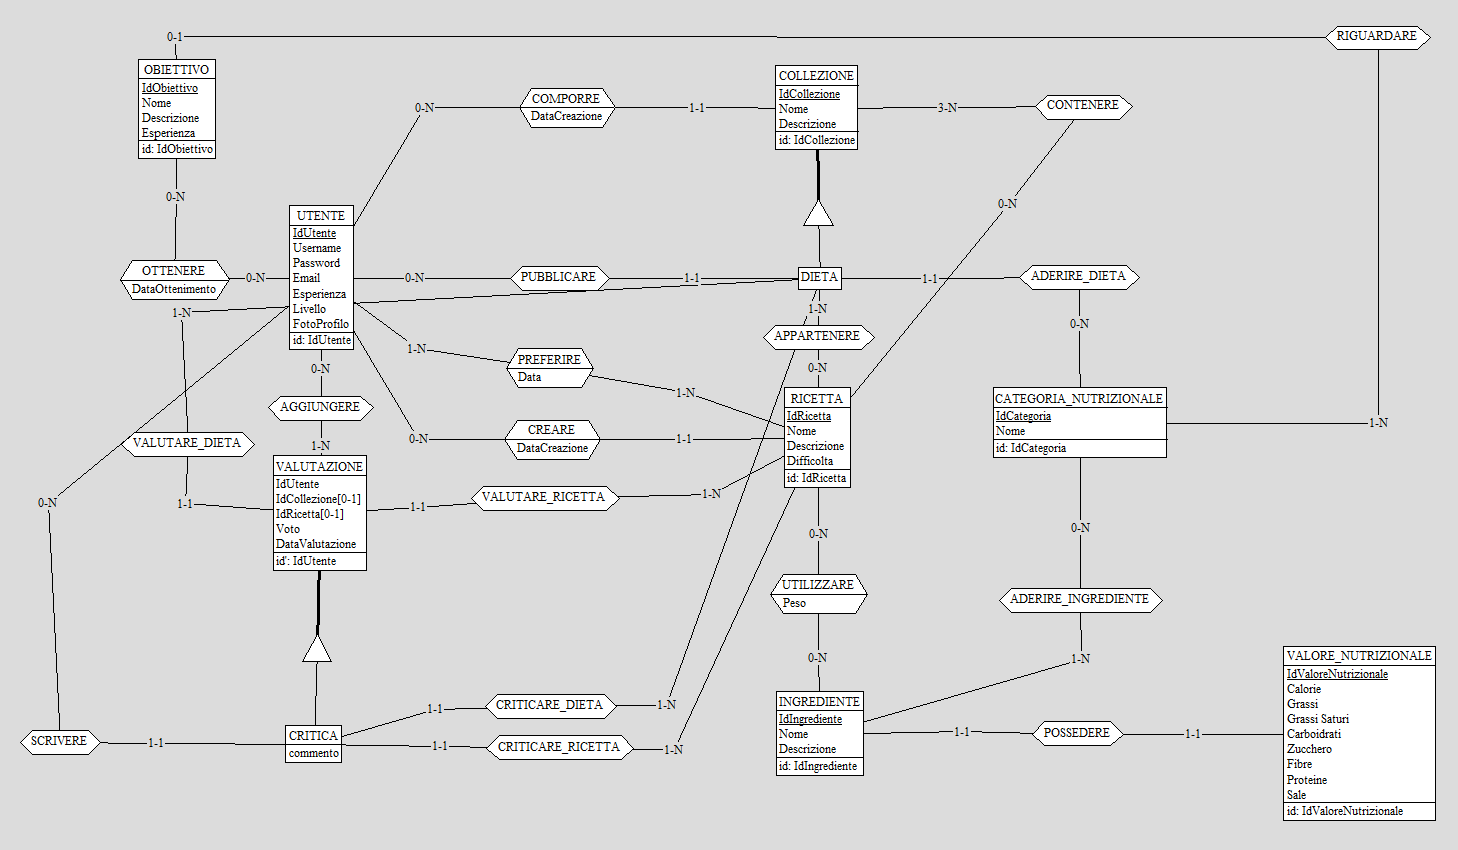
\includegraphics[width=0.9\linewidth]{schema-concettuale.png}
    \label{fig:enter-label}
\end{figure}

\subsection{Valutazione}
Per rappresentare le valutazioni e critiche
abbiamo optato per una gerarchia.
\begin{figure}[H]
    \centering
    %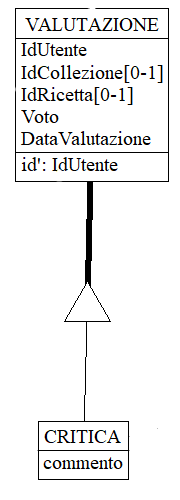
\includegraphics[width=0.2\linewidth]{valutazione-concettuale.png}
    \label{fig:enter-label}
\end{figure}
\subsection{Ingrediente}
Per rappresentare gli ingredienti abbiamo preferito separarlo in due entità, ingrediente e valori nutrizionali
\chapter{Progettazione logica}
capitolo logica
\section{Volume dei dati}
Secondo sottocapitolo
\section{Operazioni principali e frequenza}
Secondo sottocapitolo
\section{Tabelle degli accessi}
Secondo sottocapitolo
\section{Raffinamento schema}
Secondo sottocapitolo
\section{Analisi rindondanze}
Secondo sottocapitolo
\section{Traduzione di entità e relazioni in associazioni}
Secondo sottocapitolo
\section{Schema relazionale finale}
Secondo sottocapitolo
\section{Traduzione delle operazioni in query SQL}
Secondo sottocapitolo


\chapter{Progettazione applicazione}
\section{Descrizione dell'architettura\\ dell'applicazione realizzata}
Abbiamo sviluppato un'applicazione Social Media di ricette culinarie per dispositivi mobile in linguaggio C\# utilizzando il framework .NET MAUI (utilizzato per la creazione di applicazioni mobile).
Per le connesioni al database viene utilizzata la libreria C\# MySQLConnector e il database risiede in un server MySQL.
Per ogni tabella contenuta nel DB viene creata una corrispettiva classe che la rappresenta all'interno del
model dell'applicazione. Inoltre abbiamo creato una classe DBService che gestisce le connessioni effettuate al database e presenta vari metodi:
\begin{itemize}
    \item TryConnection(DBCredentials dbc): prende in input le credenziali per accedere al database e restituisce un booleano sul risultato della connessione al database.
    \item ExistInTable(string query): restituisce un booleano in base al numero di elementi che produce la query data (0 elementi prodotti = false)
    \item GetData(string query): restituisce una lista di elementi generici in base alla tabella su cui viene effettuata la query e al tipo specificato.
    \item InsertElement(List〈Tuple〈string, object〉〉 values, string query): inserisce gli elementi nella tabella specificata nella query inserendo nei valori della query non settati (?) il rispettivo valore contenuto nella lista di tuple.
    \item RemoveOrUpdateElement(string query): rimuove o aggiorna la riga di una tabella seguendo la query data.
\end{itemize}
All'avvio dell'applicazione, se si tratta del primo avvio, comparirà la schermata di Login e Registrazione.
\begin{figure}[h!]
    \begin{minipage}{.5\textwidth}
        \centering
        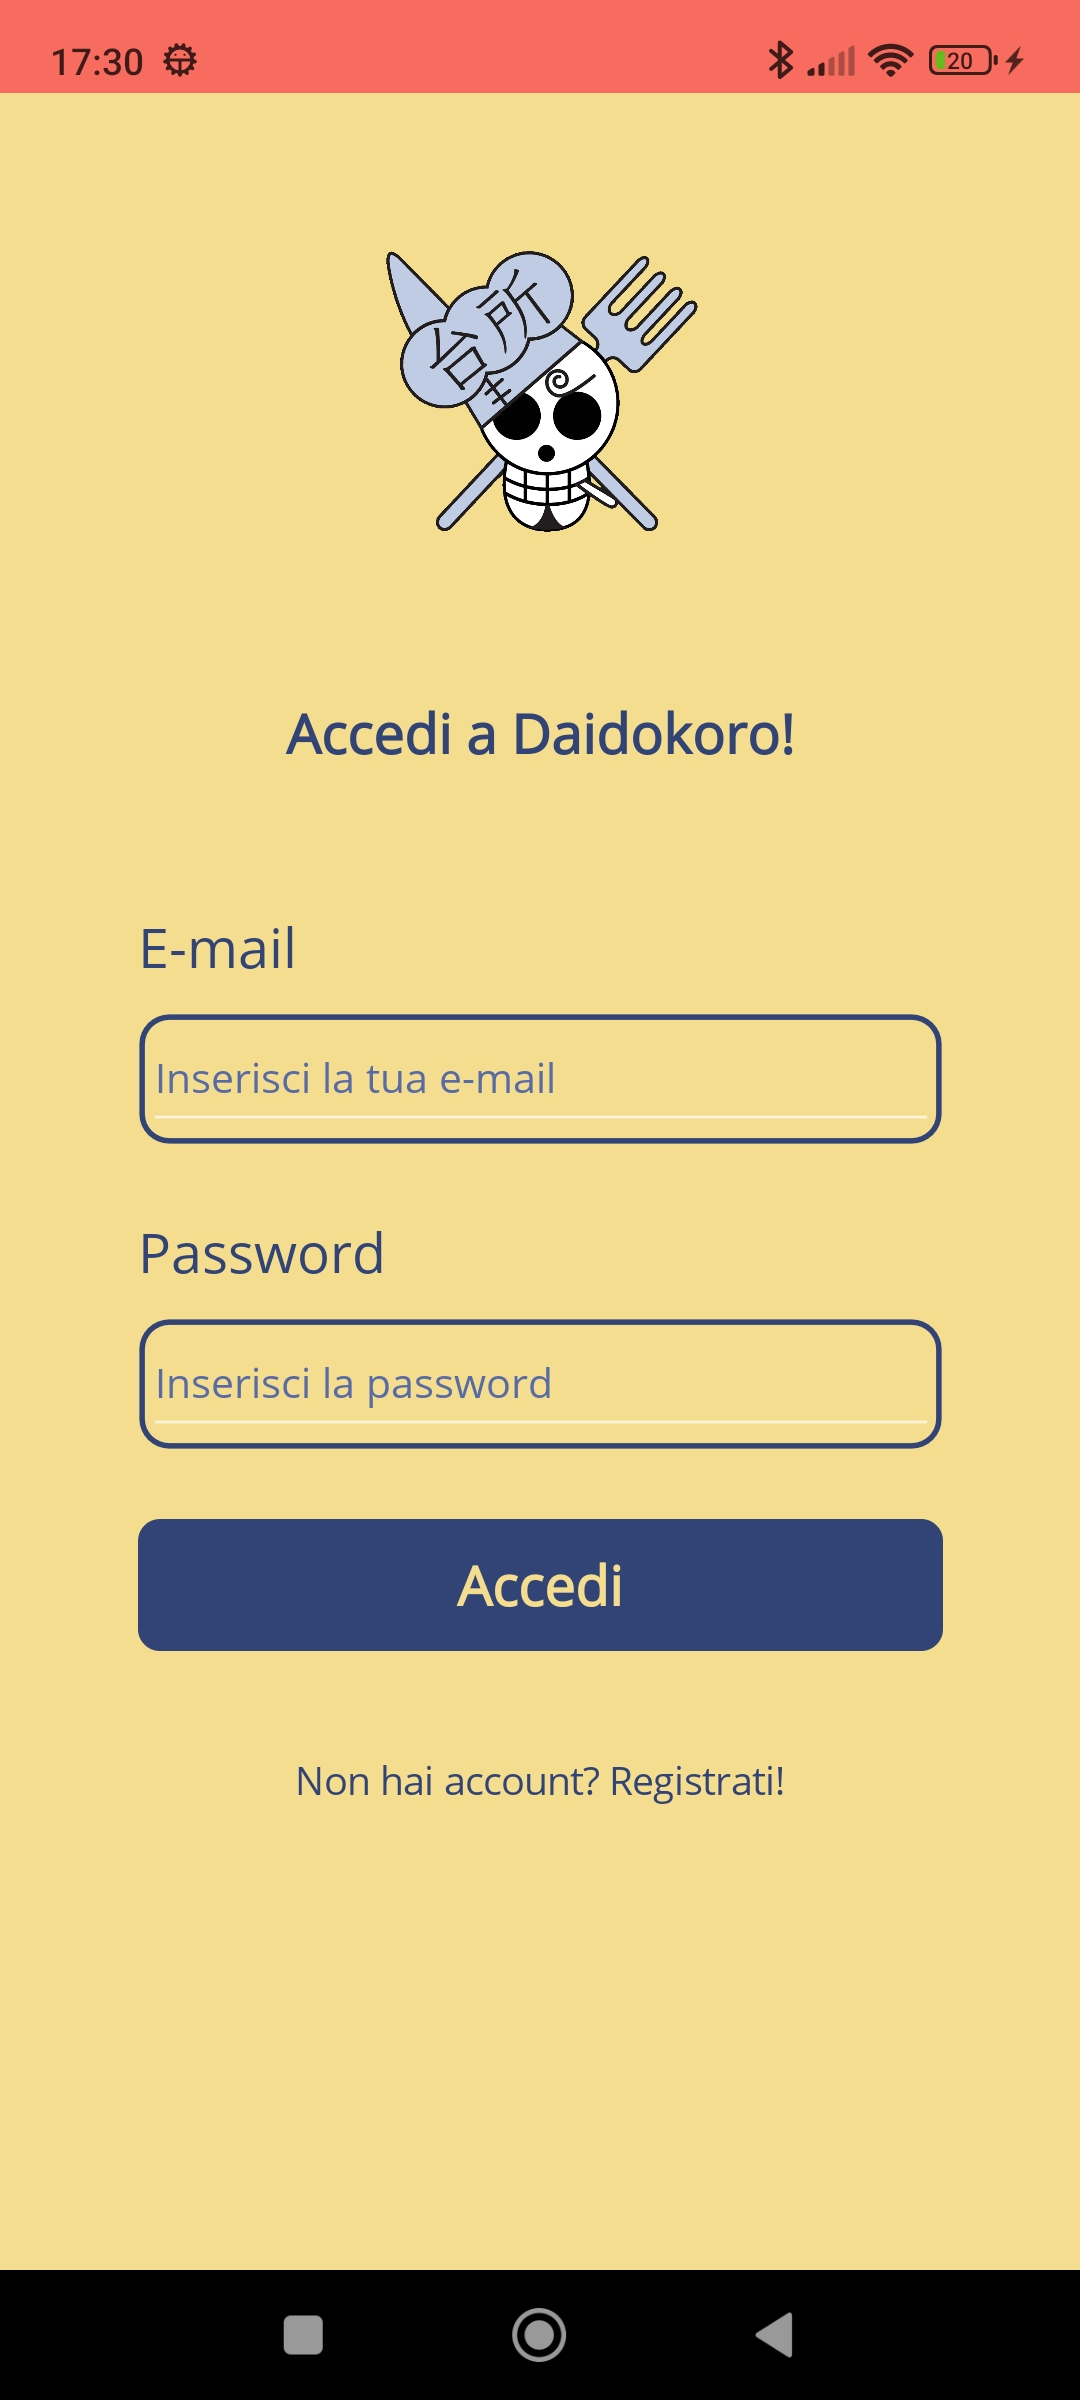
\includegraphics[width=0.9\linewidth]{app_images/Login.jpg}
    \end{minipage}
    \begin{minipage}{.5\textwidth}
        \centering
        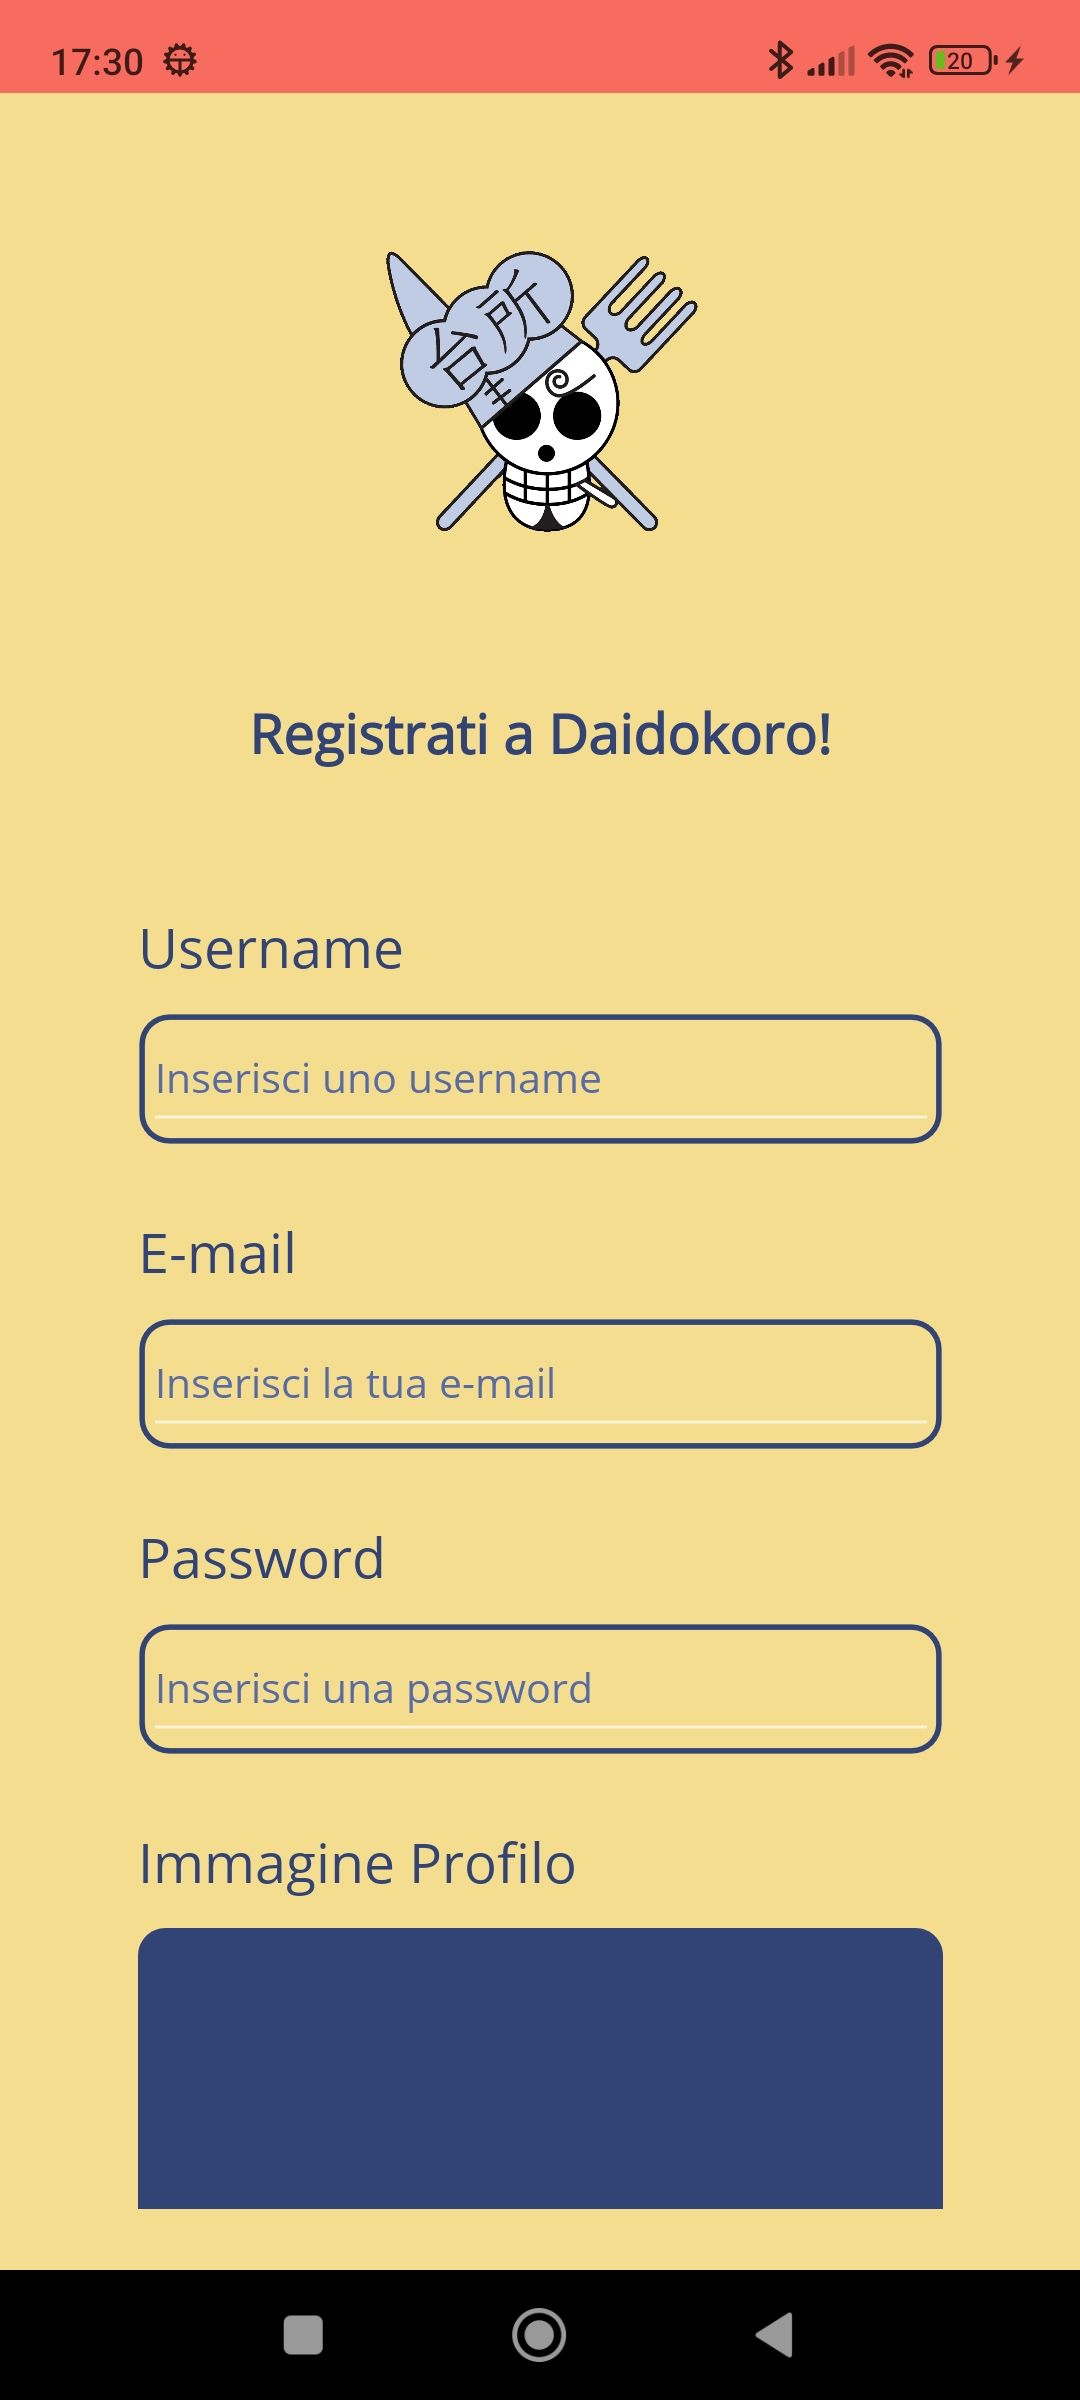
\includegraphics[width=0.9\linewidth]{app_images/Register.jpg}
    \end{minipage}
\end{figure}
\\Dopo essersi registrati e aver effettuato l'accesso verrà memorizzato nei dati dell'applicazione installata l'identificativo dell'utente che ha effettuato l'accesso in modo da poter reindirizzare l'utente sulla schermata principale ad ogni avvio successivo dell'app e caricare i suoi dati.
\\\\\\\\\\\\\\Nella Home Page è possibile visualizzare le 3 ricette con più like.
\\Clickando, invece, sull'icona centrale del menu di navigazione sovrastante, si potrà andare sulla pagina di navigazione delle ricette, collezioni e diete
\begin{figure}[h!]
    \begin{minipage}{.5\textwidth}
        \centering
        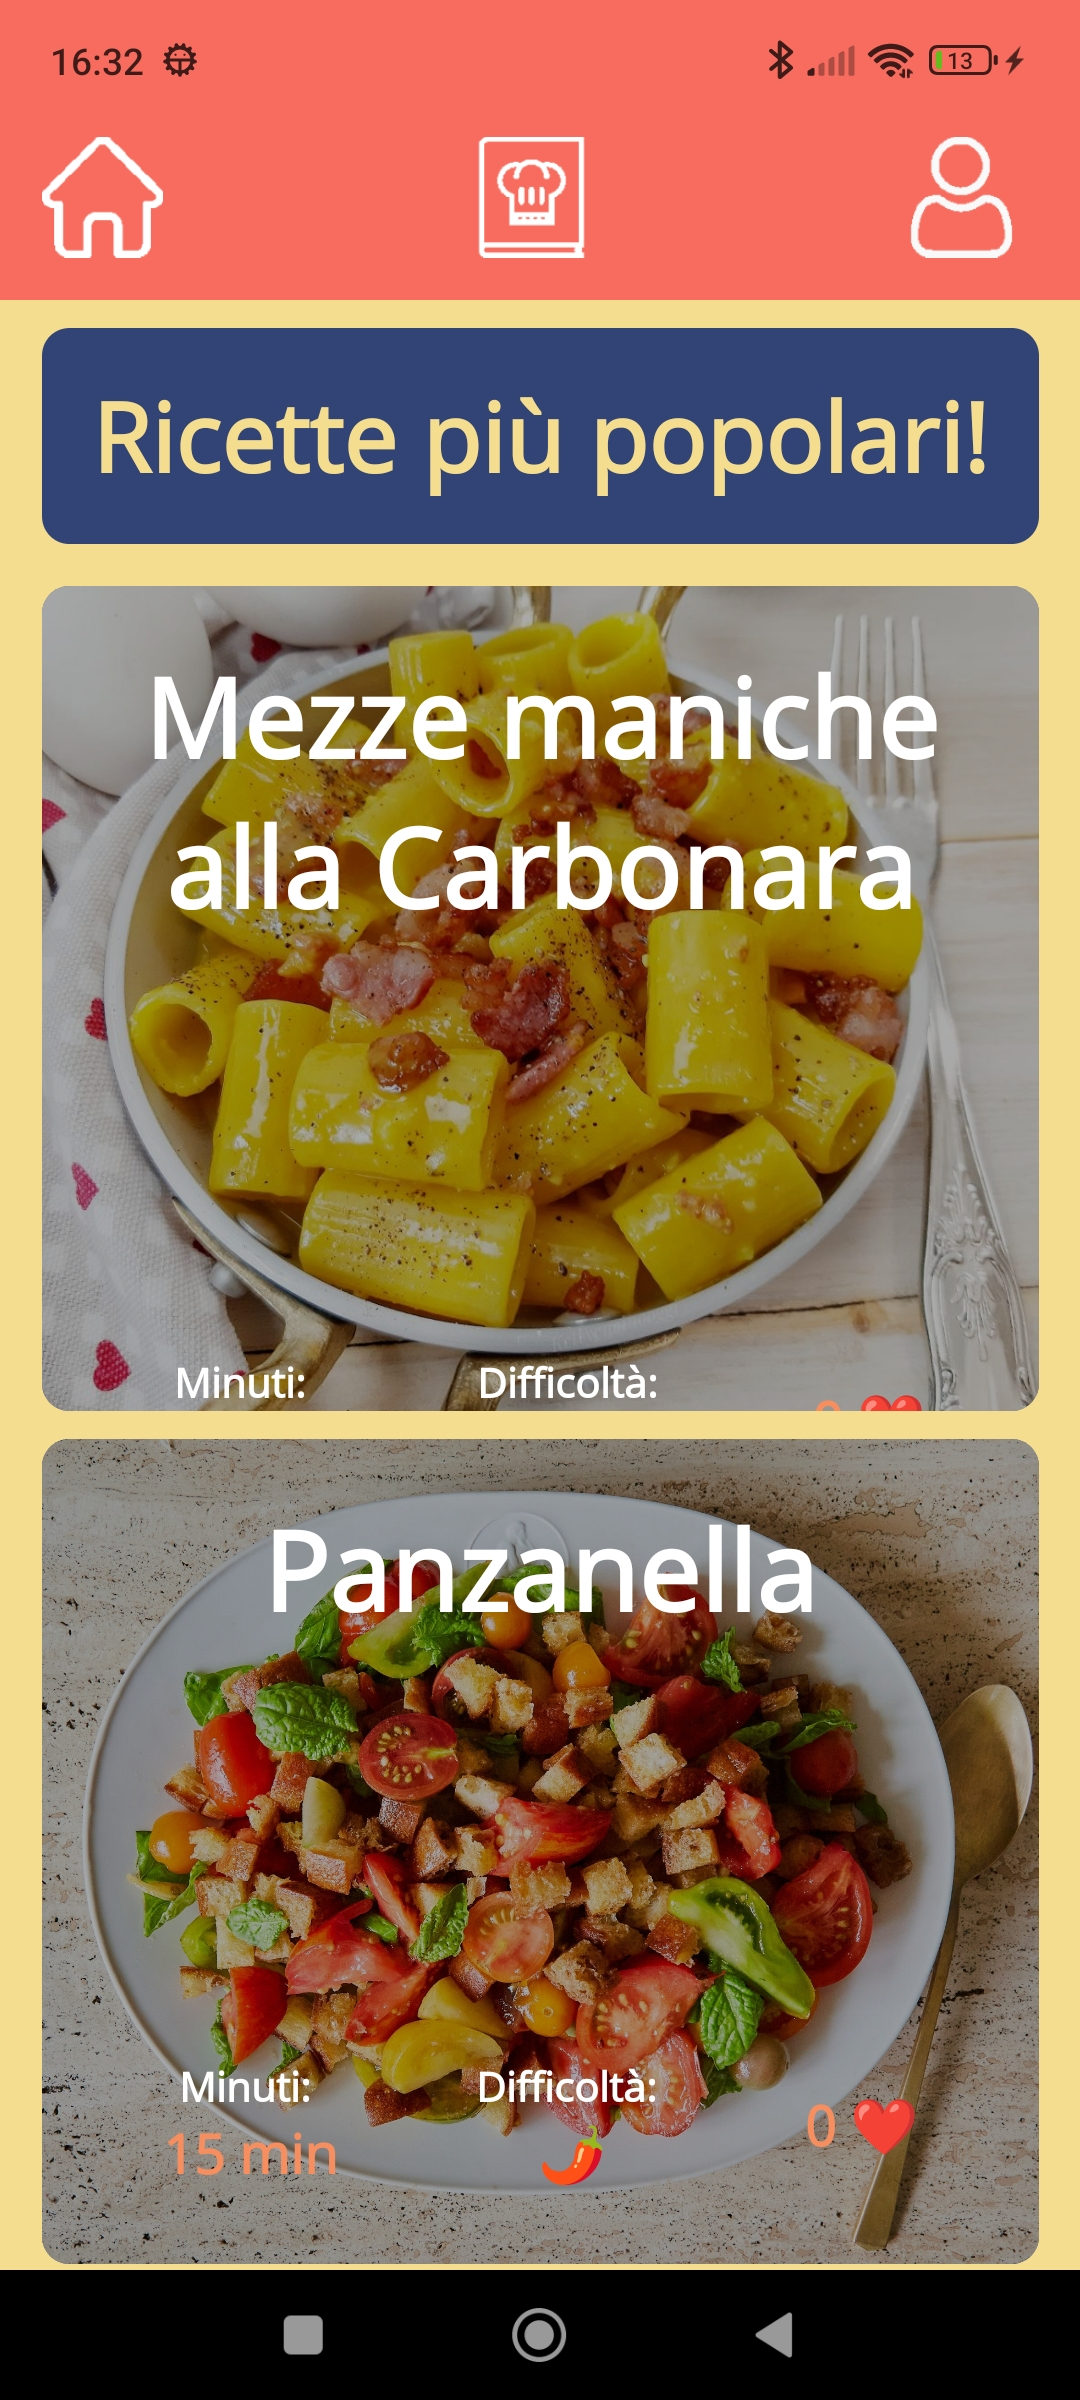
\includegraphics[width=0.9\linewidth]{app_images/HomePage.jpg}
    \end{minipage}
    \begin{minipage}{.5\textwidth}
        \centering
        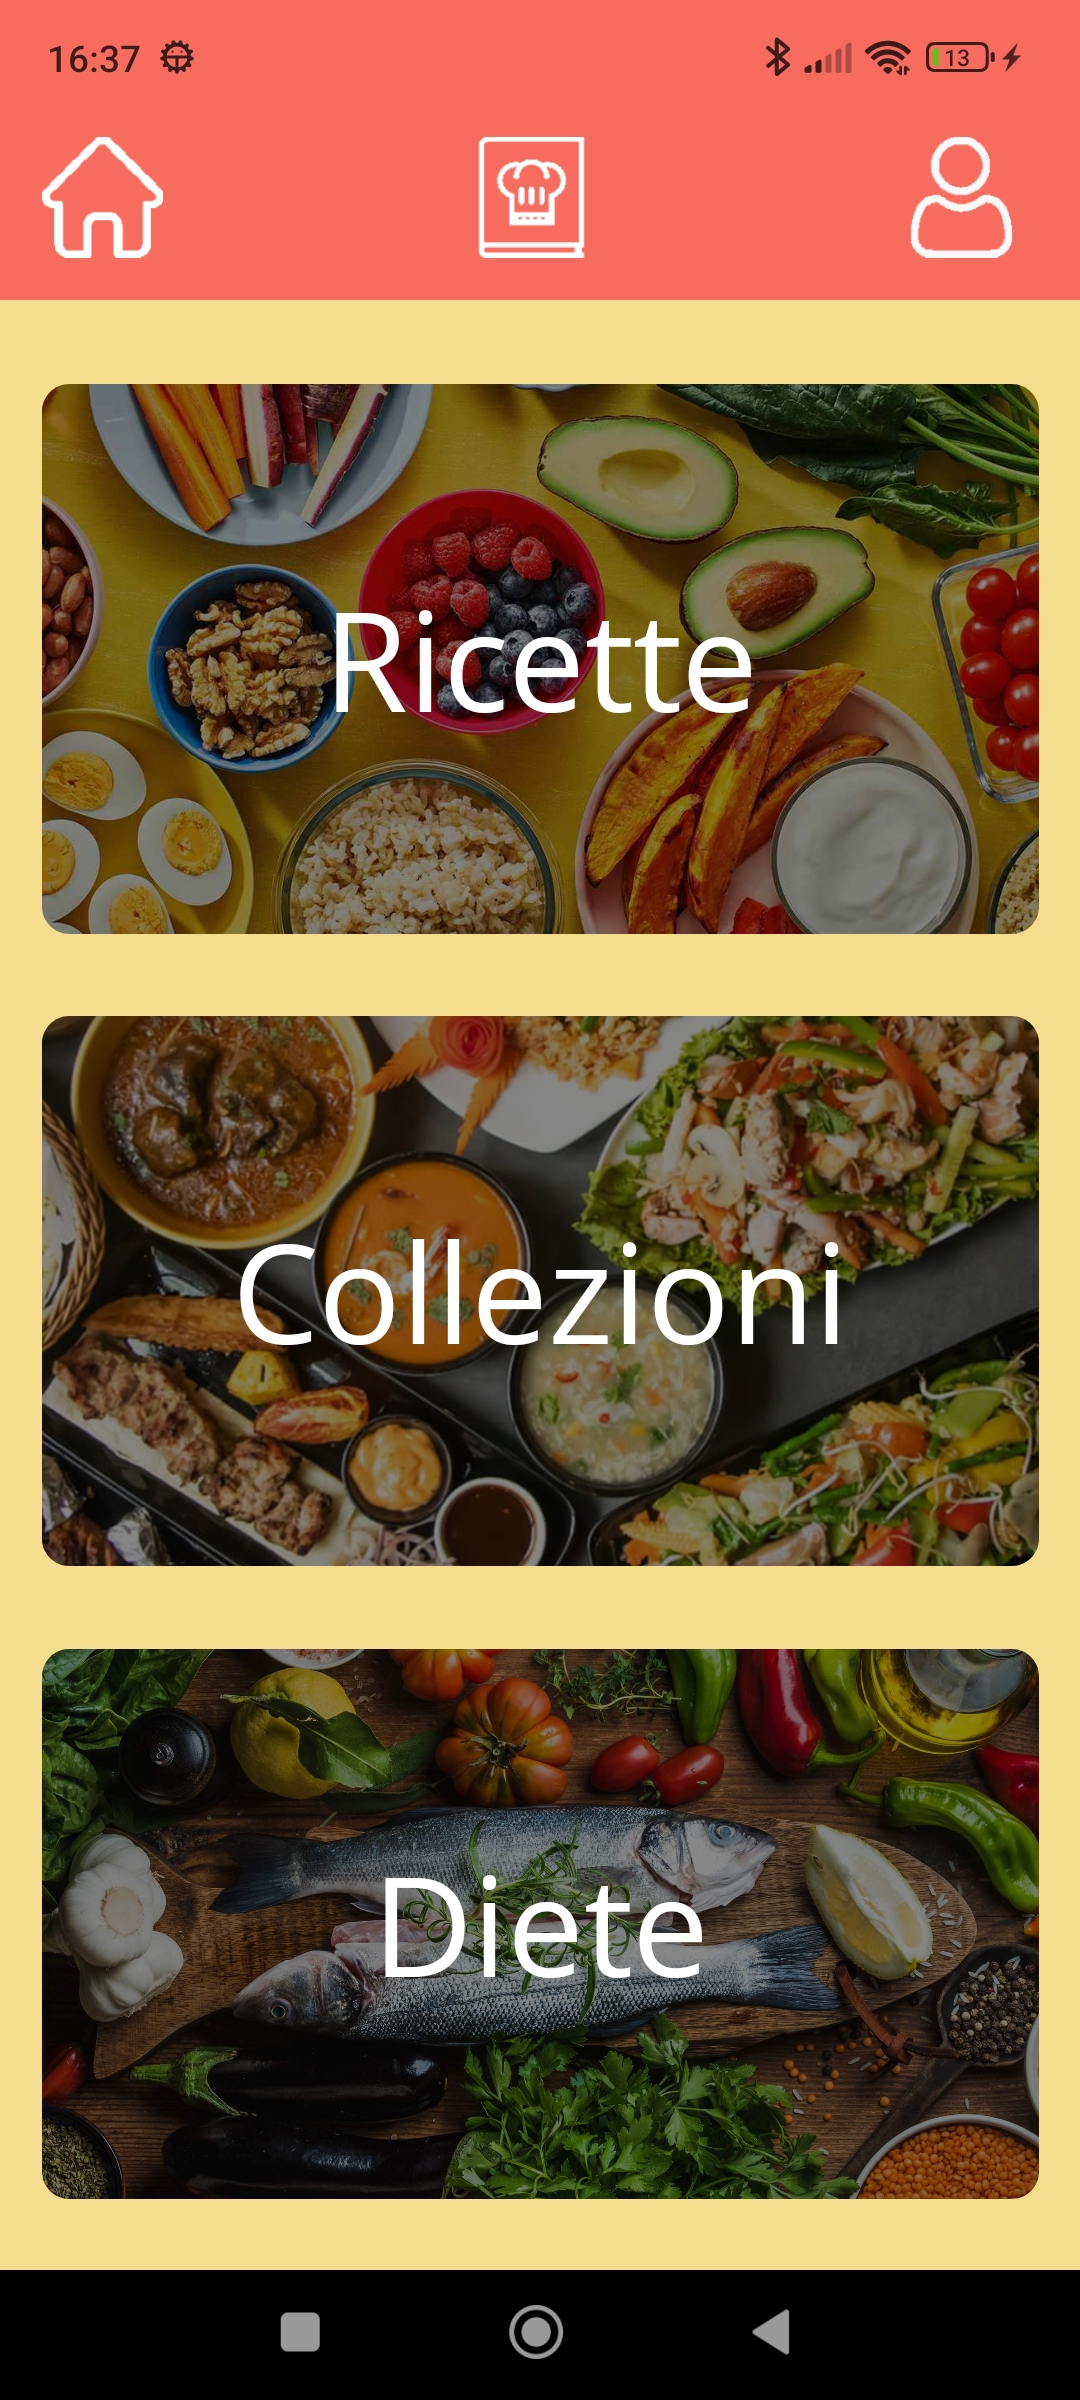
\includegraphics[width=0.9\linewidth]{app_images/BrowsePage.jpg}
    \end{minipage}
\end{figure}
\\Successivamente nella pagina di navigazione in base all'elemento clickato comparirà la pagina di visualizzazione della lista del rispetto elemento.
\\\\\\\\Di seguito si ha a sinistra la pagina con la lista delle ricette di qualunque utente con la rispettiva barra di ricerca e filtri.
Mentre a destra la pagina con la lista di collezioni di qualunque utente e la barra di ricerca.
\begin{figure}[h!]
    \begin{minipage}{.5\textwidth}
        \centering
        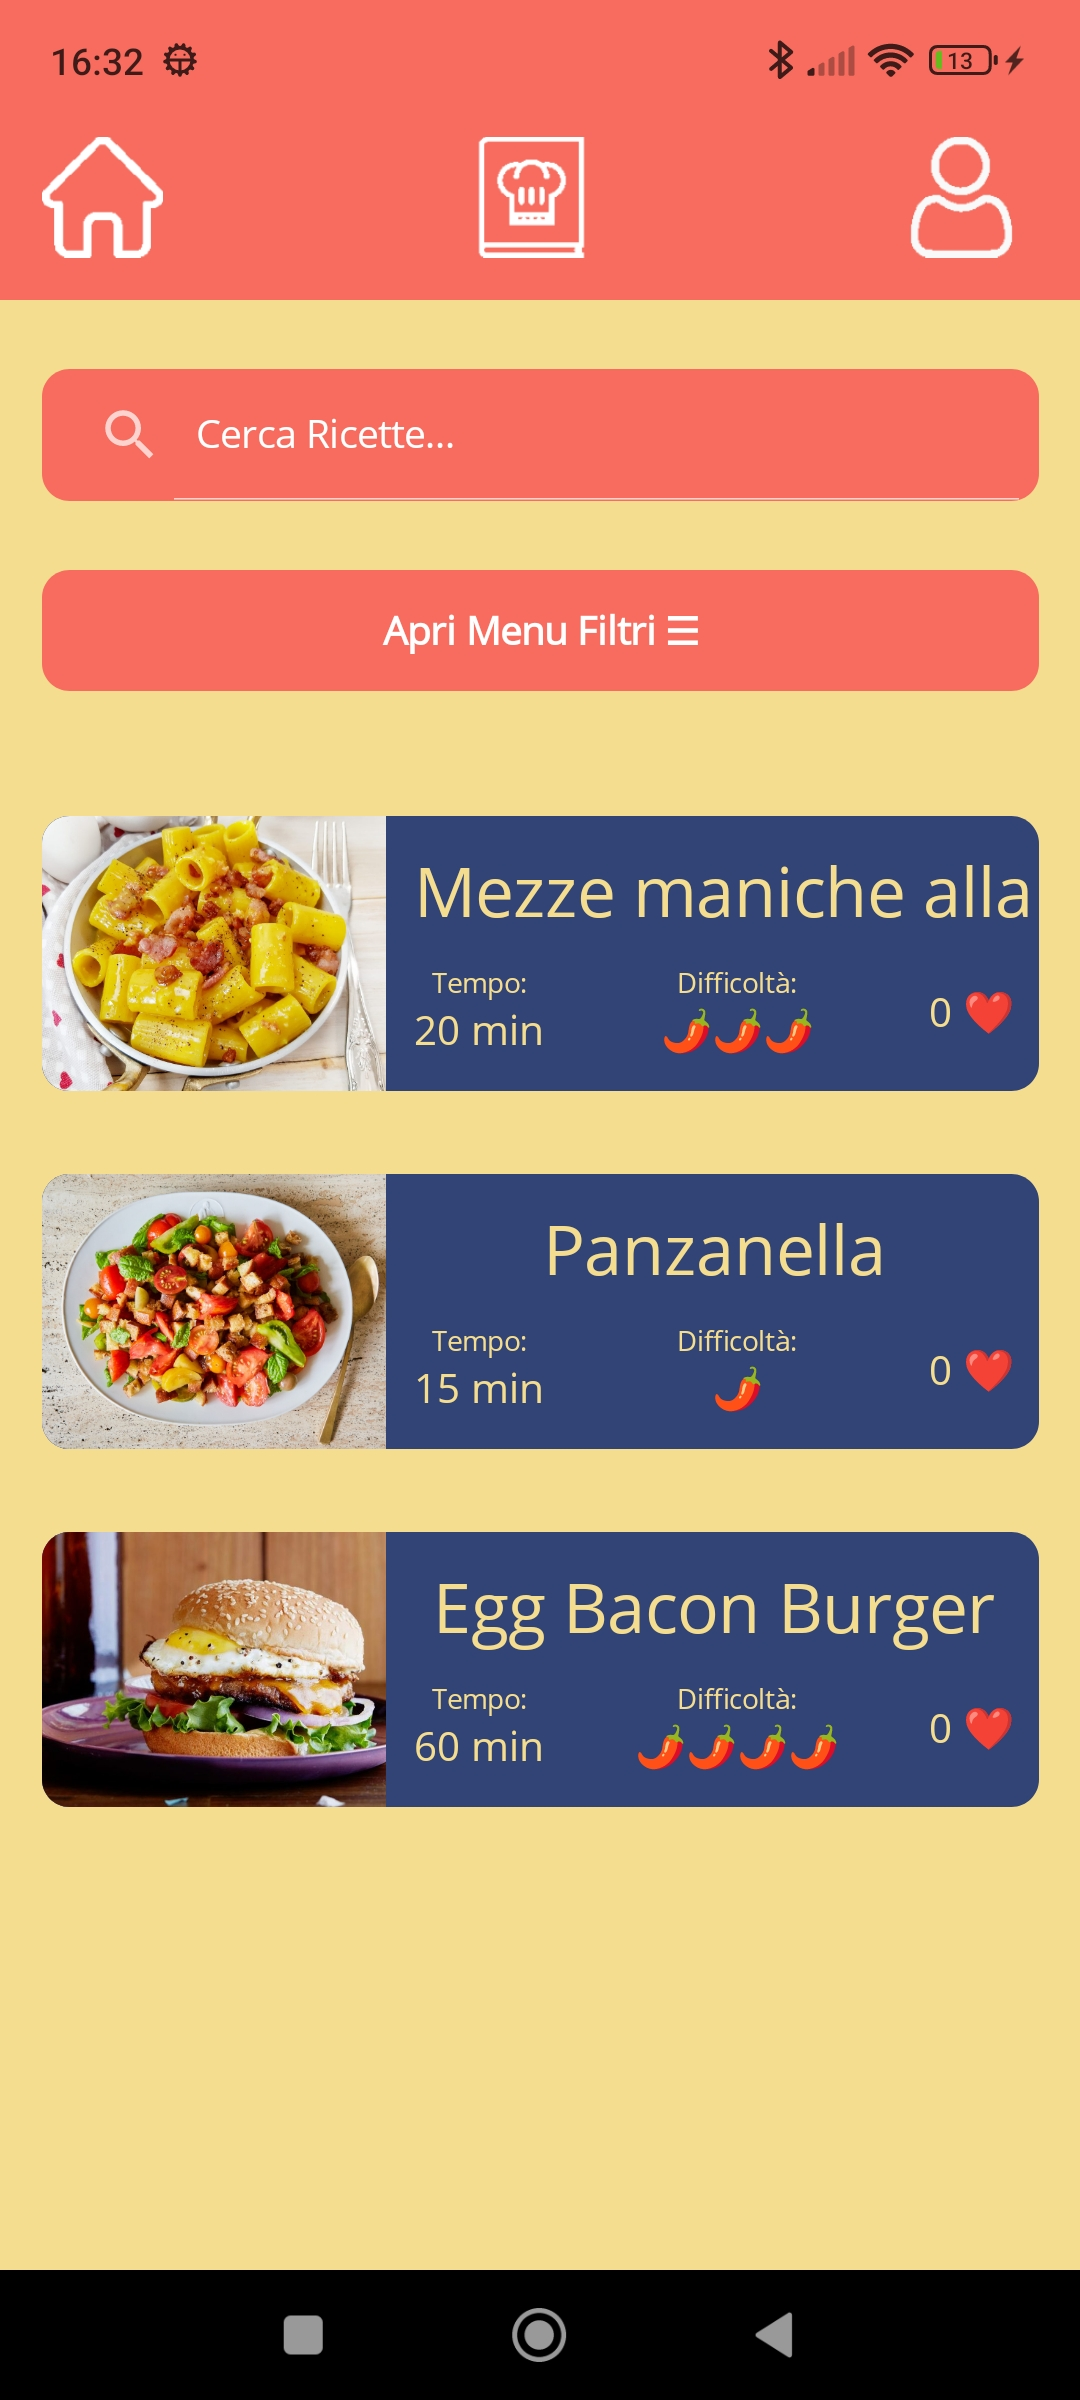
\includegraphics[width=0.9\linewidth]{app_images/RecipeList.jpg}
    \end{minipage}
    \begin{minipage}{.5\textwidth}
        \centering
        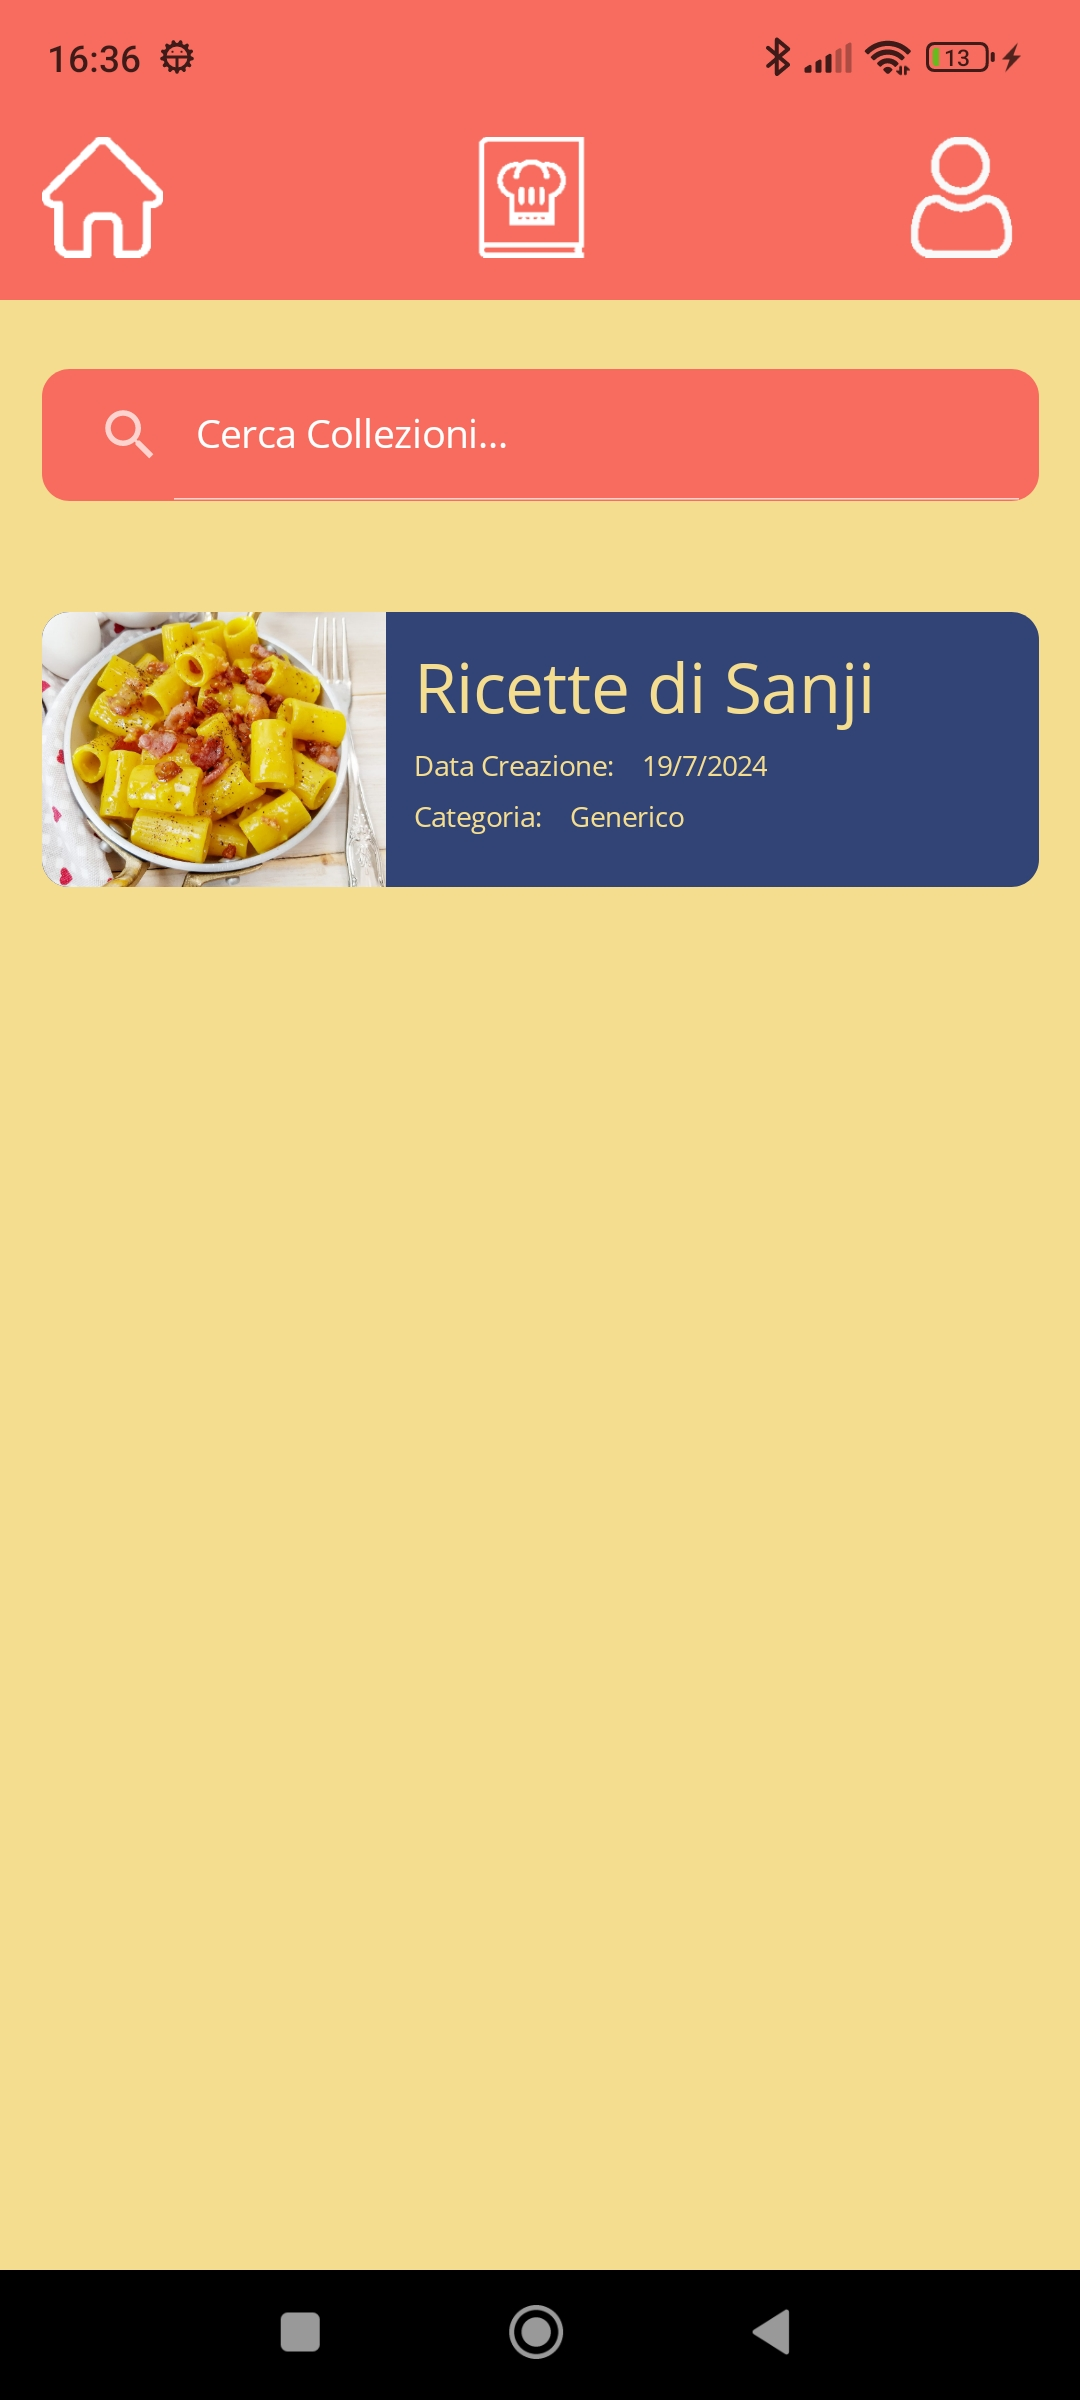
\includegraphics[width=0.9\linewidth]{app_images/CollectionList.jpg}
    \end{minipage}
\end{figure}
\\\\Ogni ricetta nella lista presenta l'immagine, il nome, il tempo di preparazione, difficoltà rappresentata da 1 a 5 con l'emoji di un peperoncino e il numero di like ricevuti da utenti.
Mentre le collezioni avranno come immagine quella della ricetta con più like nella collezione, la data di creazione e la categoria.
\\\\La pagina delle diete è composta come quella delle collezioni ma presente un menu dei filtri come quello delle ricette oltre alla barra di ricerca.
\begin{figure}[h!]
    \begin{minipage}{.5\textwidth}
        \centering
        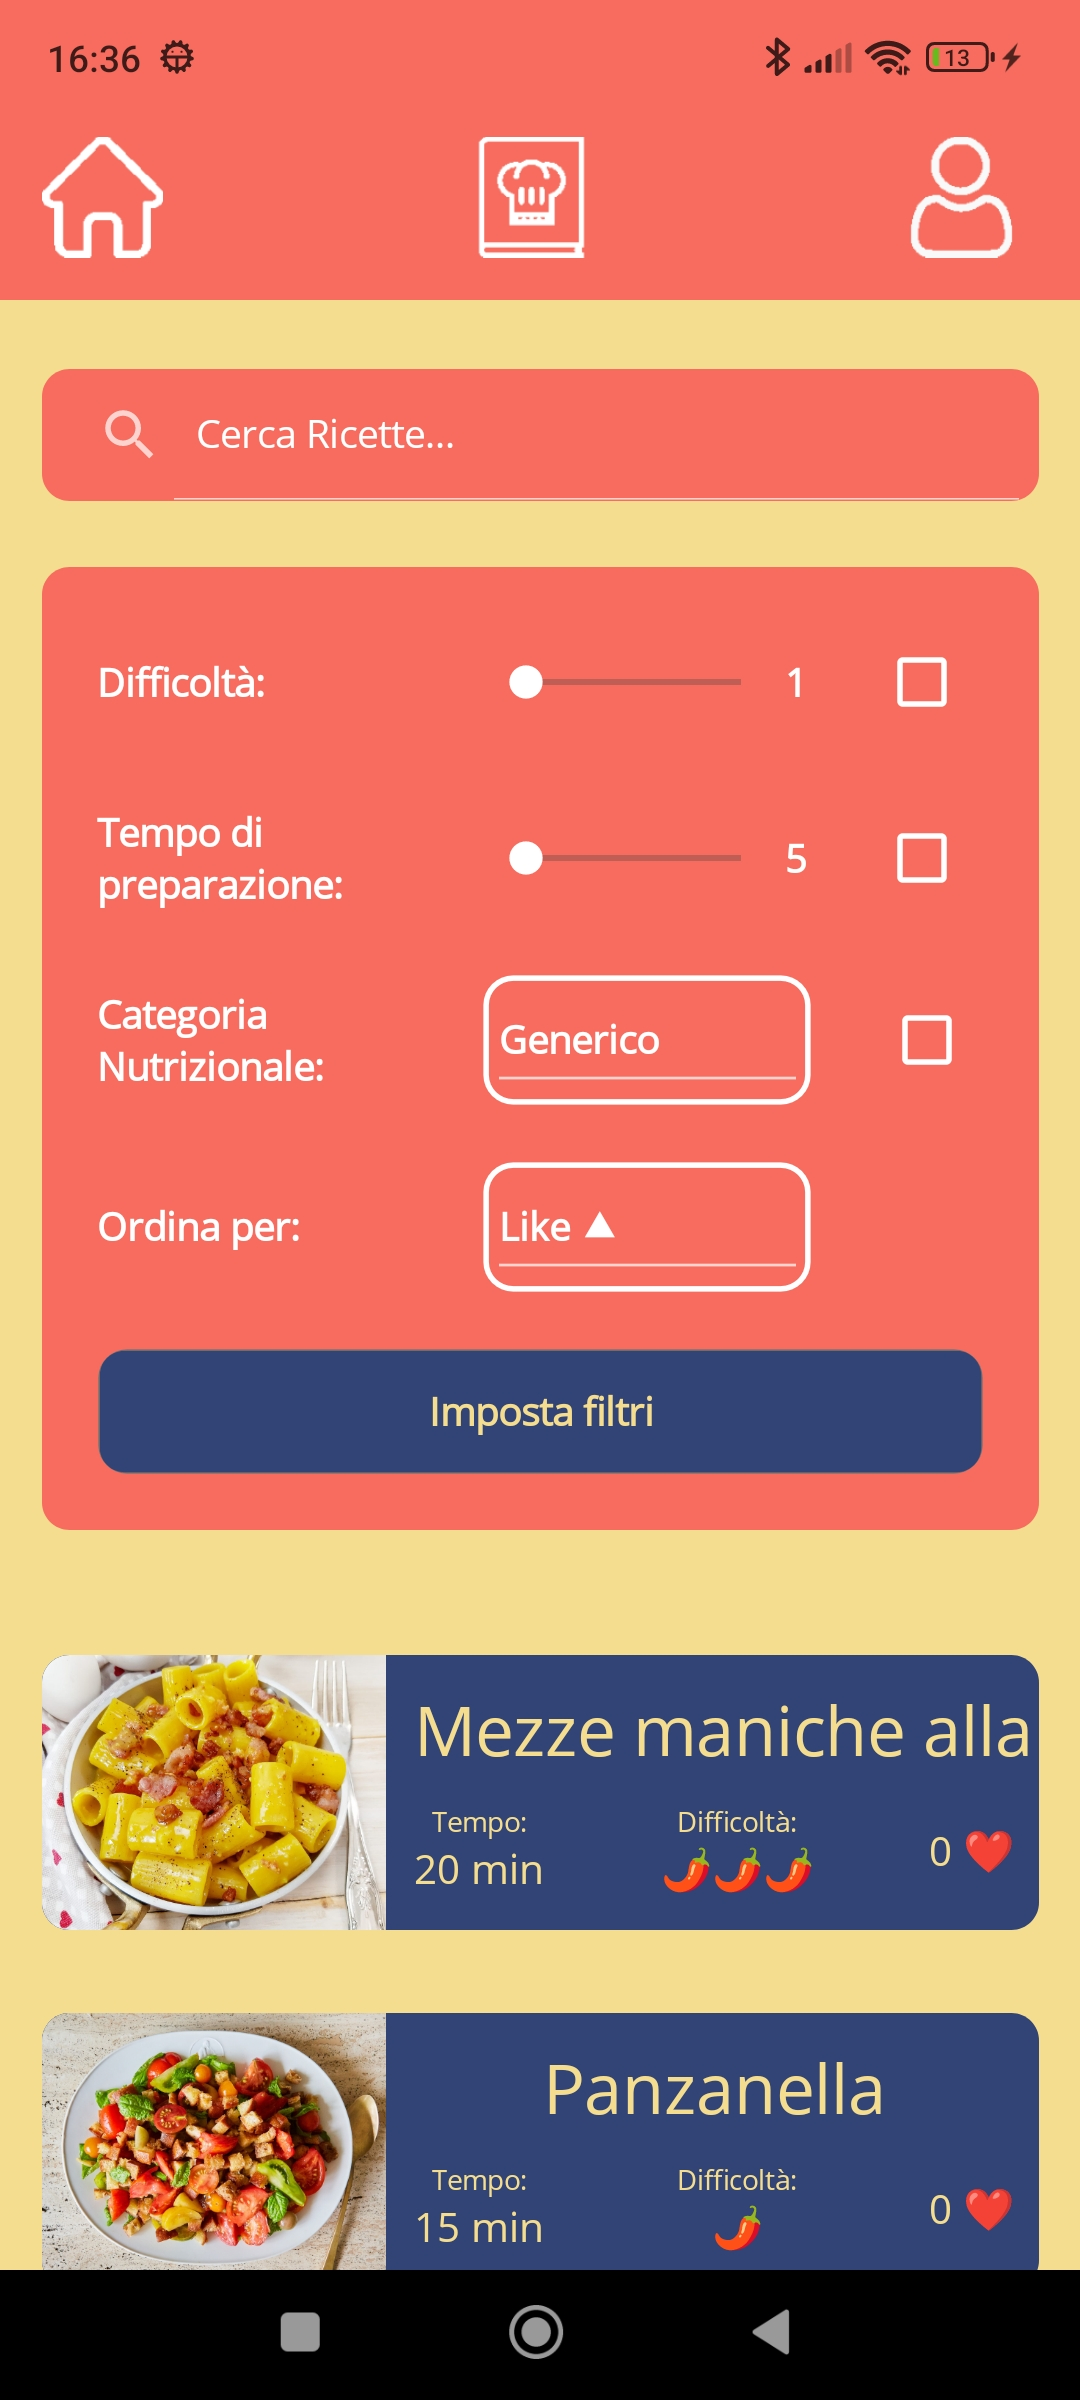
\includegraphics[width=0.9\linewidth]{app_images/Filter.jpg}
    \end{minipage}
    \begin{minipage}{.5\textwidth}
        \centering
        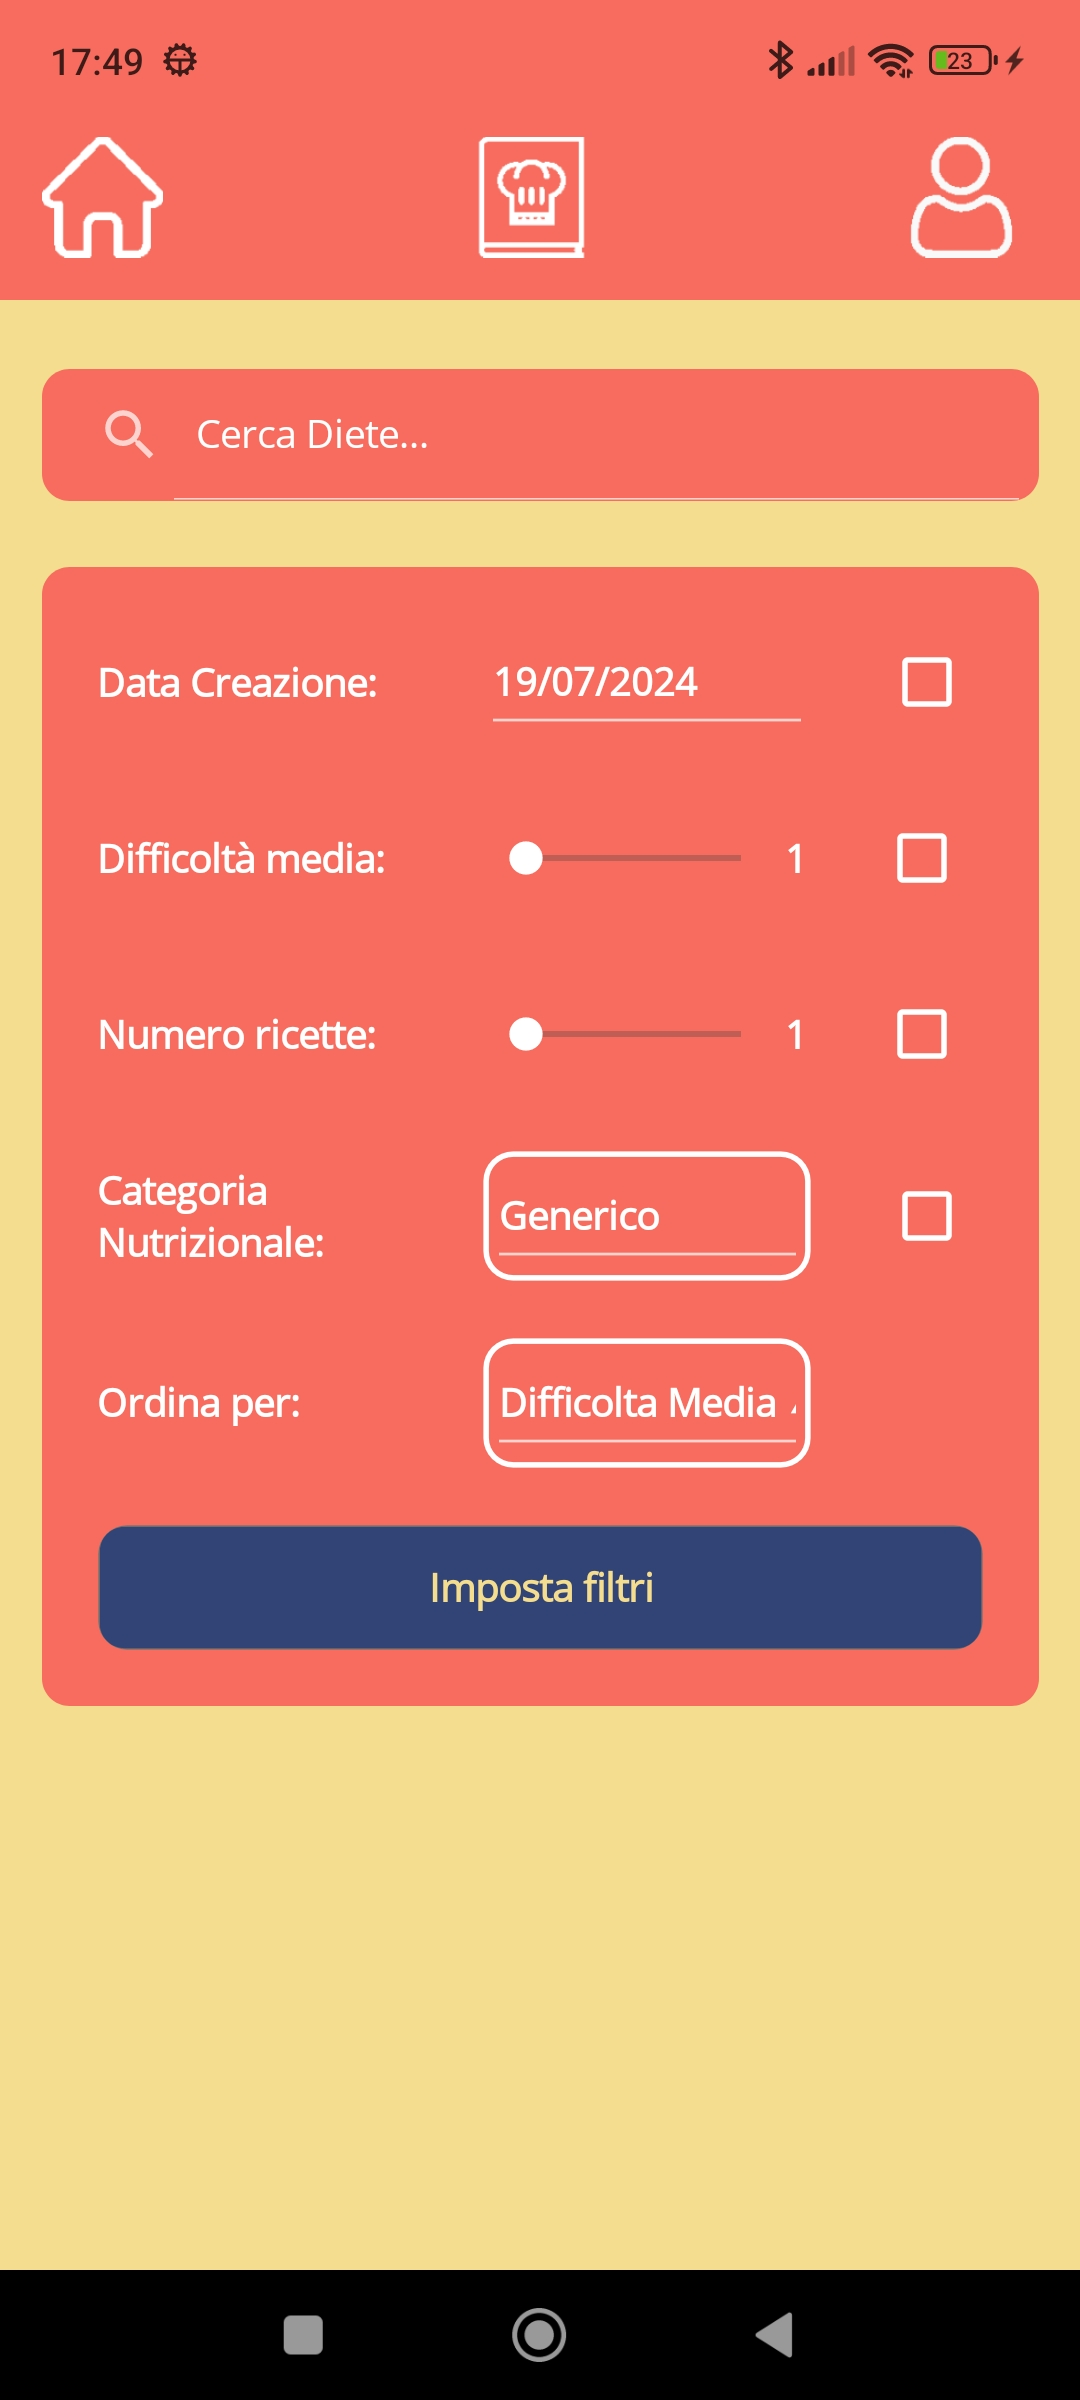
\includegraphics[width=0.9\linewidth]{app_images/Filter2.jpg}
    \end{minipage}
\end{figure}
\\La barra di ricerca delle diete effettuerà la ricerca di una ricetta in base al nome, al nome degli ingredienti associati e al nome della categoria nutrizionale degli ingredienti, mentre quella delle collezioni e delle diete cercherà in base al nome della collezione/dieta e al nome delle ricette contenute.
\\\\Per quanto riguarda le ricette, il menu dei filtri contiene uno slider per la difficoltà e uno per il tempo di preparazione, un selettore per la categoria nutrizionale e un selettore per l'ordinamento da effettuare sulle ricette filtrate.
Mentre il menu dei filtri delle diete contiene un selettore per la data di creazione, uno slider per la difficoltà media delle ricette contenute nella dieta, uno slider per il numero massimo di ricette nella dieta e i due selettori per la categoria nutrizionale della dieta e l'ordinamento sulle diete filtrate.
\\\\\\\\\\Quando si va su una delle pagine contenenti le liste di elementi, clickando su un elemento si andrà alla pagina del singolo elemento con tutte le informazioni specifiche. 
Di seguito si ha la pagina di una ricetta.
\begin{figure}[h!]
    \begin{minipage}{.5\textwidth}
        \centering
        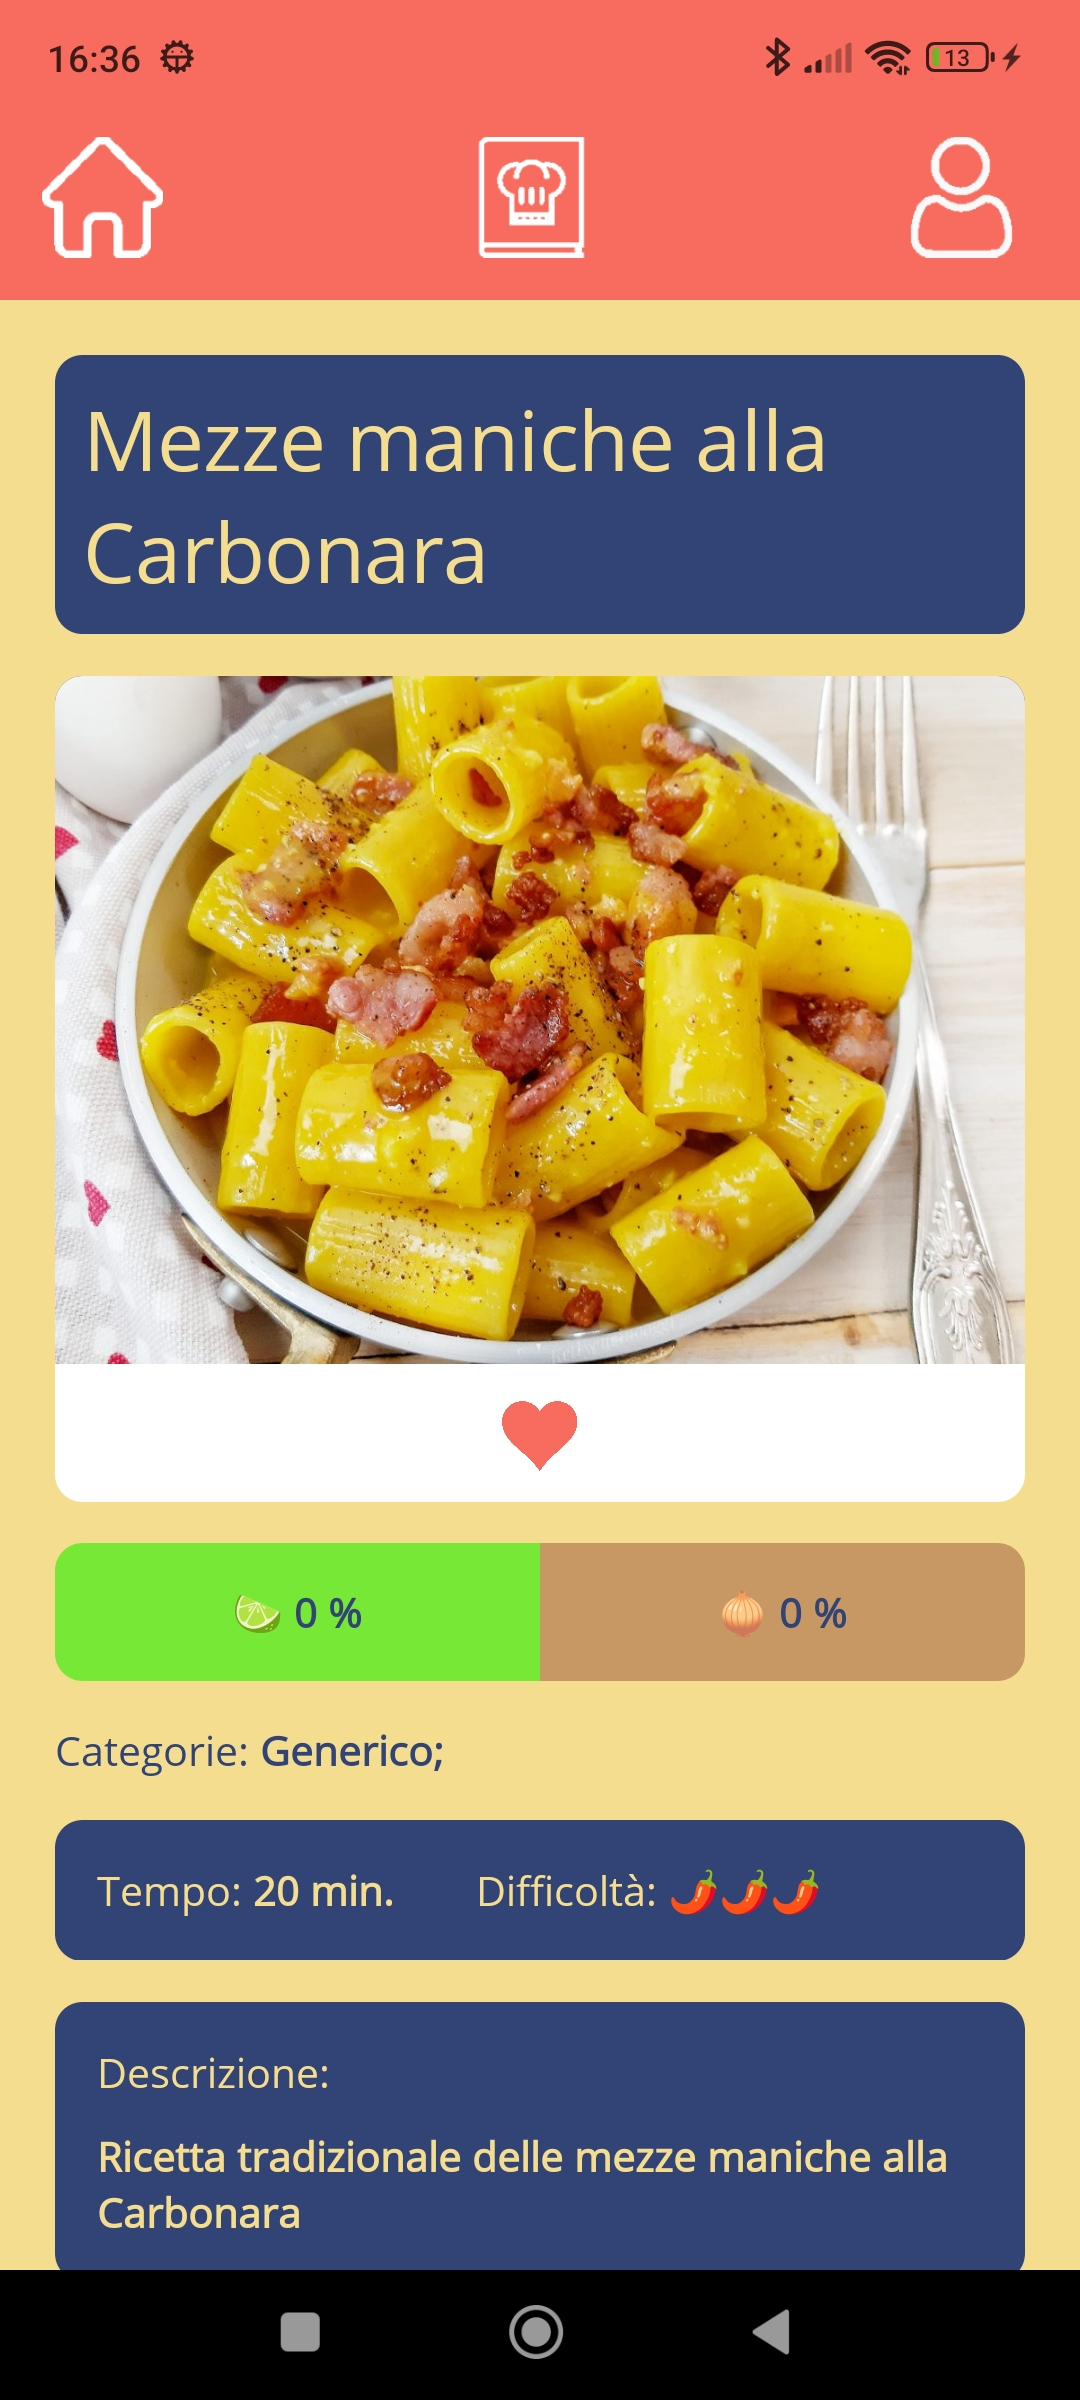
\includegraphics[width=0.9\linewidth]{app_images/Liked.jpg}
    \end{minipage}
    \begin{minipage}{.5\textwidth}
        \centering
        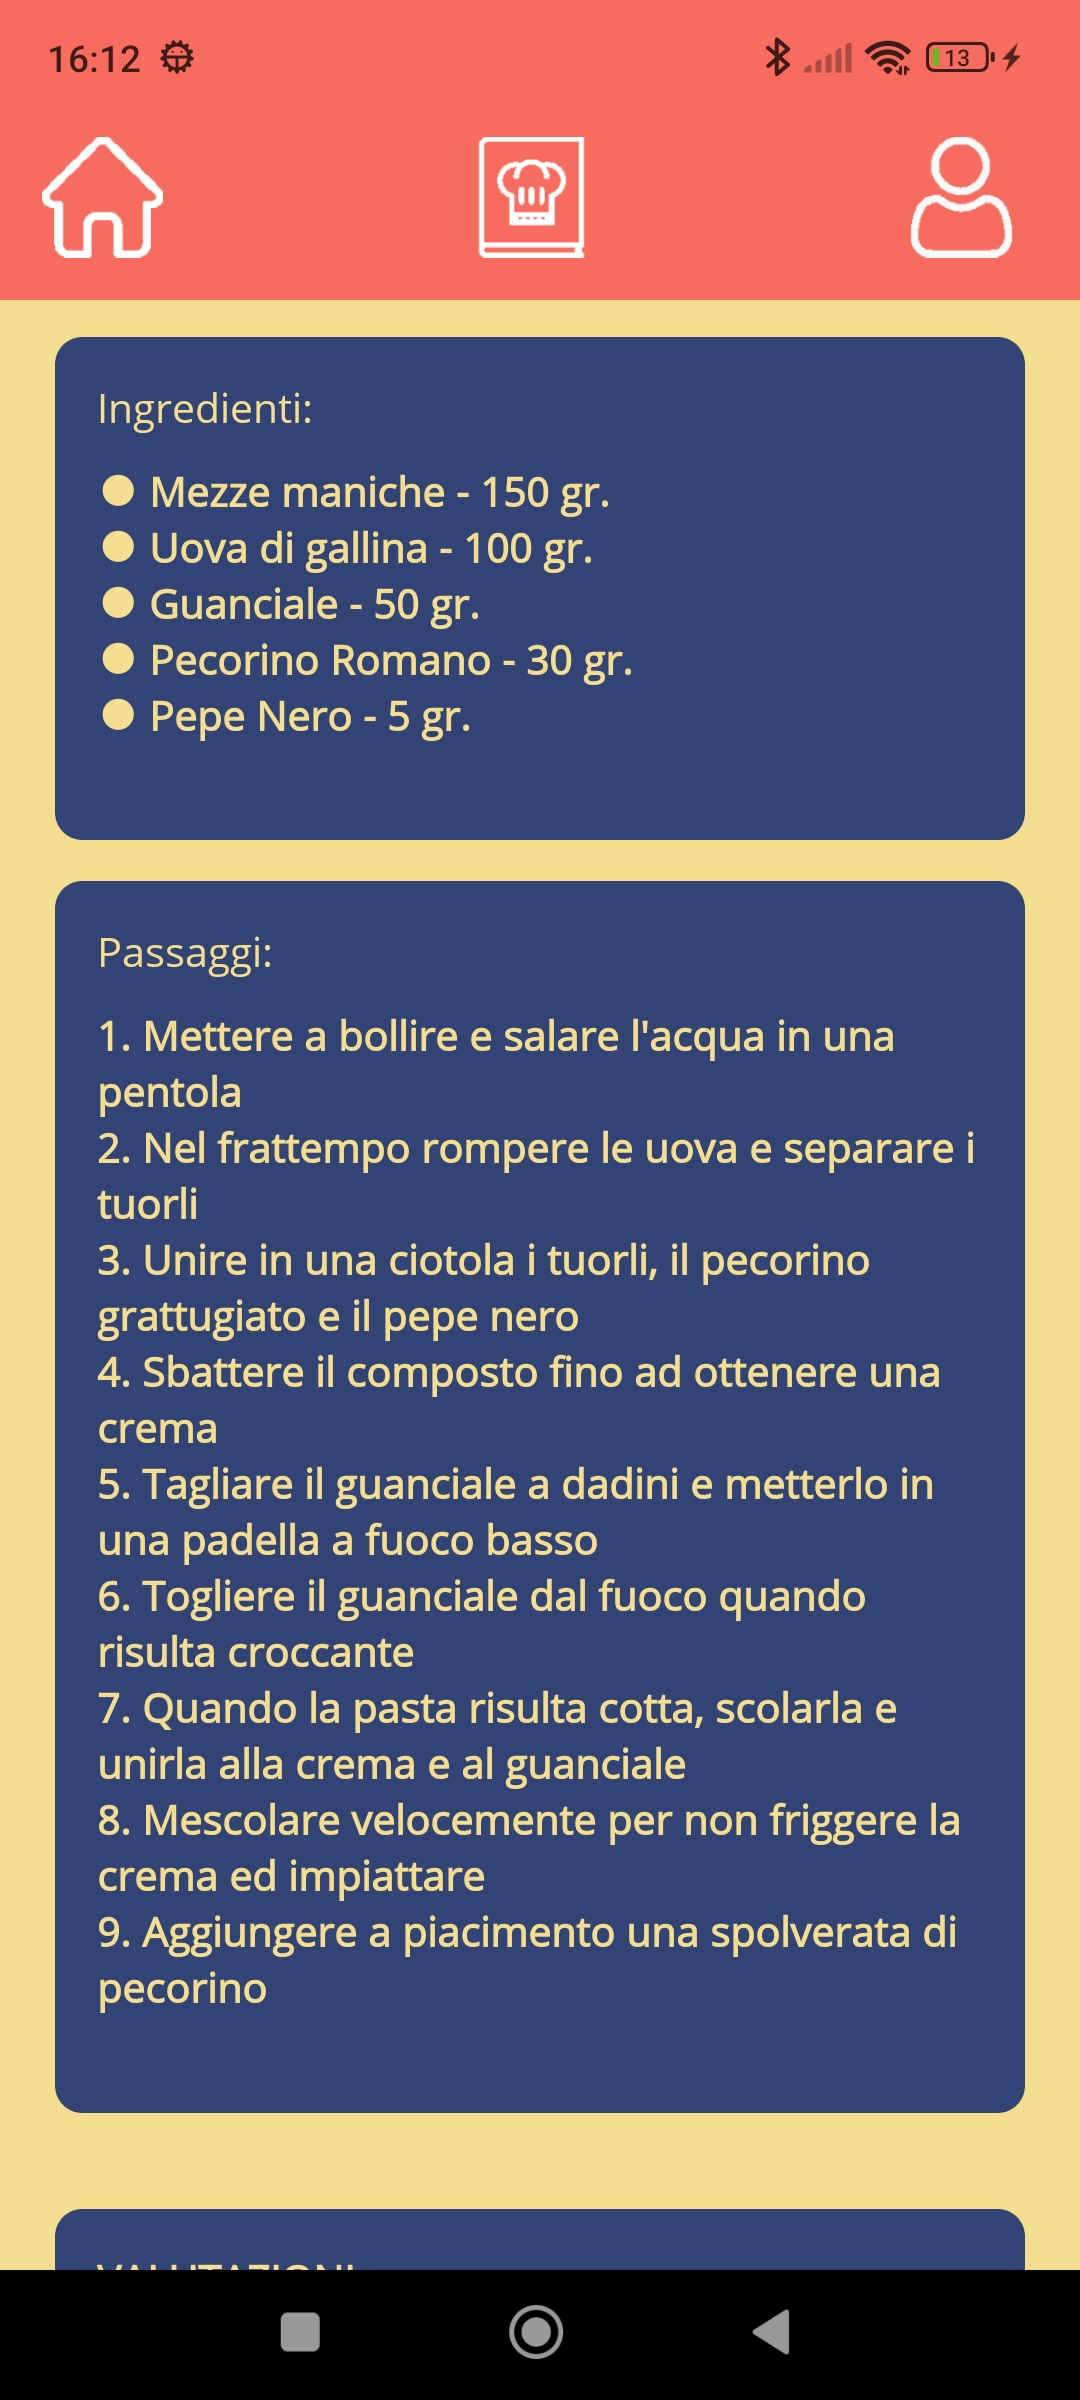
\includegraphics[width=0.9\linewidth]{app_images/RecipePage2.jpg}
    \end{minipage}
\end{figure}
\\In questa pagina l'utente potrà visualizzare tutte le informazioni della ricetta come la descrizione, gli ingredienti e i passaggi.
Inoltre potrà aggiungere la ricetta ai preferiti clickando sul pulsante con il cuore e potrà valutare la ricetta con un voto positivo (\colorbox{LimeGreen}{\textbf{Lime}}) o negativo (\colorbox{Tan}{\textbf{Cipolla}}).
In fondo alla pagina l'utente troverà la sezione delle valutazioni dove compariranno tutte le valutazioni degli utenti e l'utente potrà aggiungere un commento alla valutazione effettuata in precedenza.
\\\\\\Nella pagina della singola collezione/dieta, invece, si ha inizialmente una sezione con le informazioni principali, seguita dagli stessi bottoni per le valutazioni come nella pagina delle ricette e la lista delle ricette contenute nella collezione/dieta.
In fondo alla pagina si ha la sezione delle valutazioni con la possibilità di inserire il commento come per le ricette, nella pagina di una dieta però il commento può essere inserito solo se si ha sbloccato l'obiettivo della categoria nutrizionale a cui appartiene la dieta.
\begin{figure}[h!]
    \begin{minipage}{.5\textwidth}
        \centering
        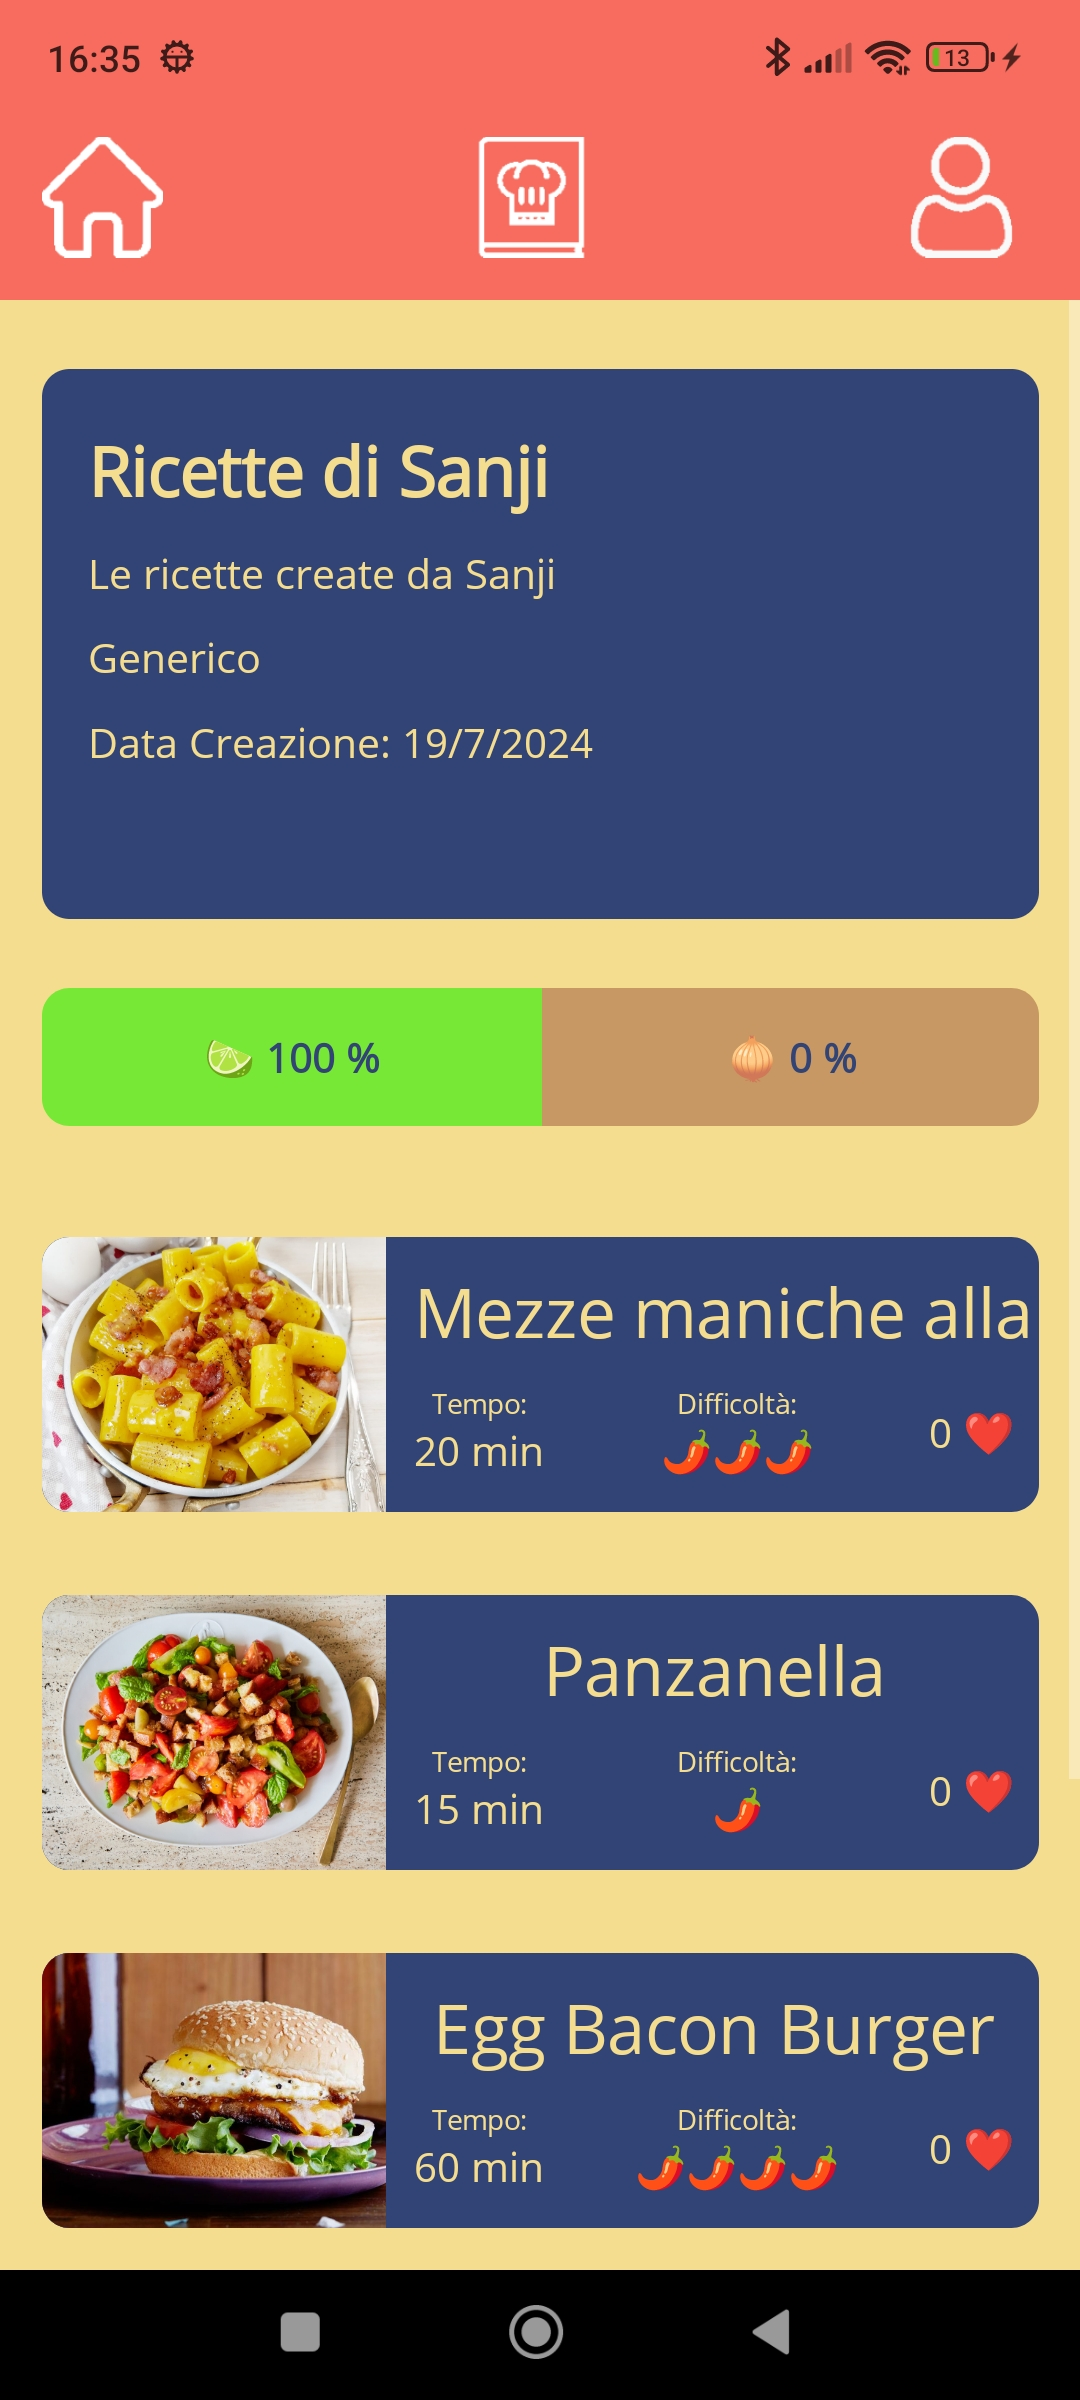
\includegraphics[width=0.9\linewidth]{app_images/CollectionPage.jpg}
    \end{minipage}
    \begin{minipage}{.5\textwidth}
        \centering
        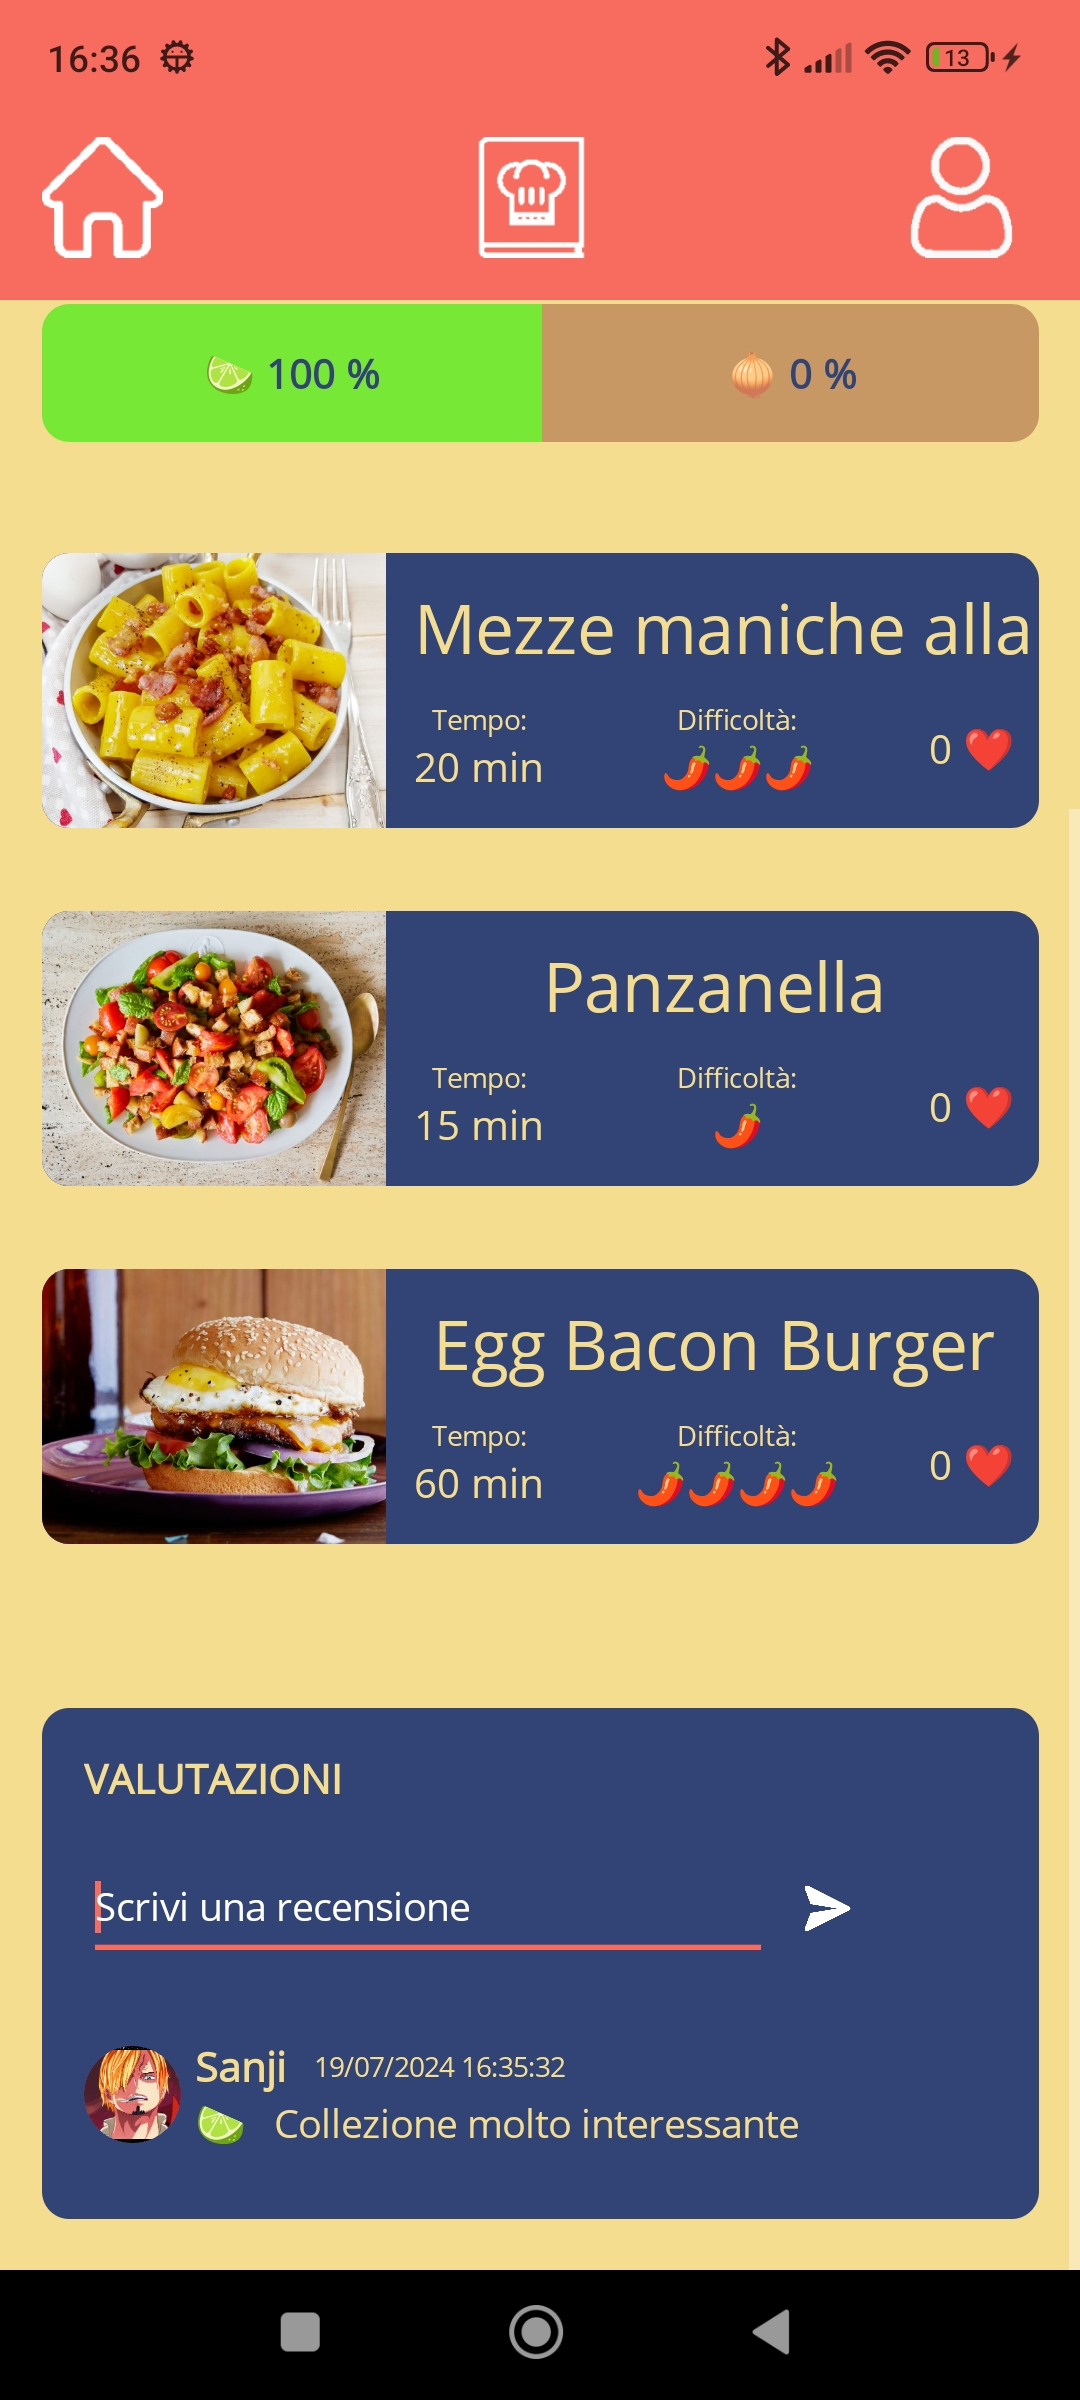
\includegraphics[width=0.9\linewidth]{app_images/CollectionPage2.jpg}
    \end{minipage}
\end{figure}
\\\\\\\\Tornando sul menu sovrastante di navigazione, clickando sull'icona a destra si andrà sulla propria pagina utente.
\\In questa pagina si ha la foto profilo inserita in fase di registrazione e il nome, seguiti da il tasto per effettuare il logout e i seguenti contatori delle statistiche dell'utente:
\begin{itemize}
    \item Numero di ricette create
    \item Numero di collezioni create
    \item Numero di recensioni create
    \item Numero di ricette aggiunte ai preferiti
    \item Numero di obiettivi ottenuti
\end{itemize}
Infine si hanno i pulsanti per la creazione di ricette e collezioni e una lista dove, al click di un contatore, compariranno gli elementi a cui fa riferimento quel contatore.
\begin{figure}[h!]
    \centering
    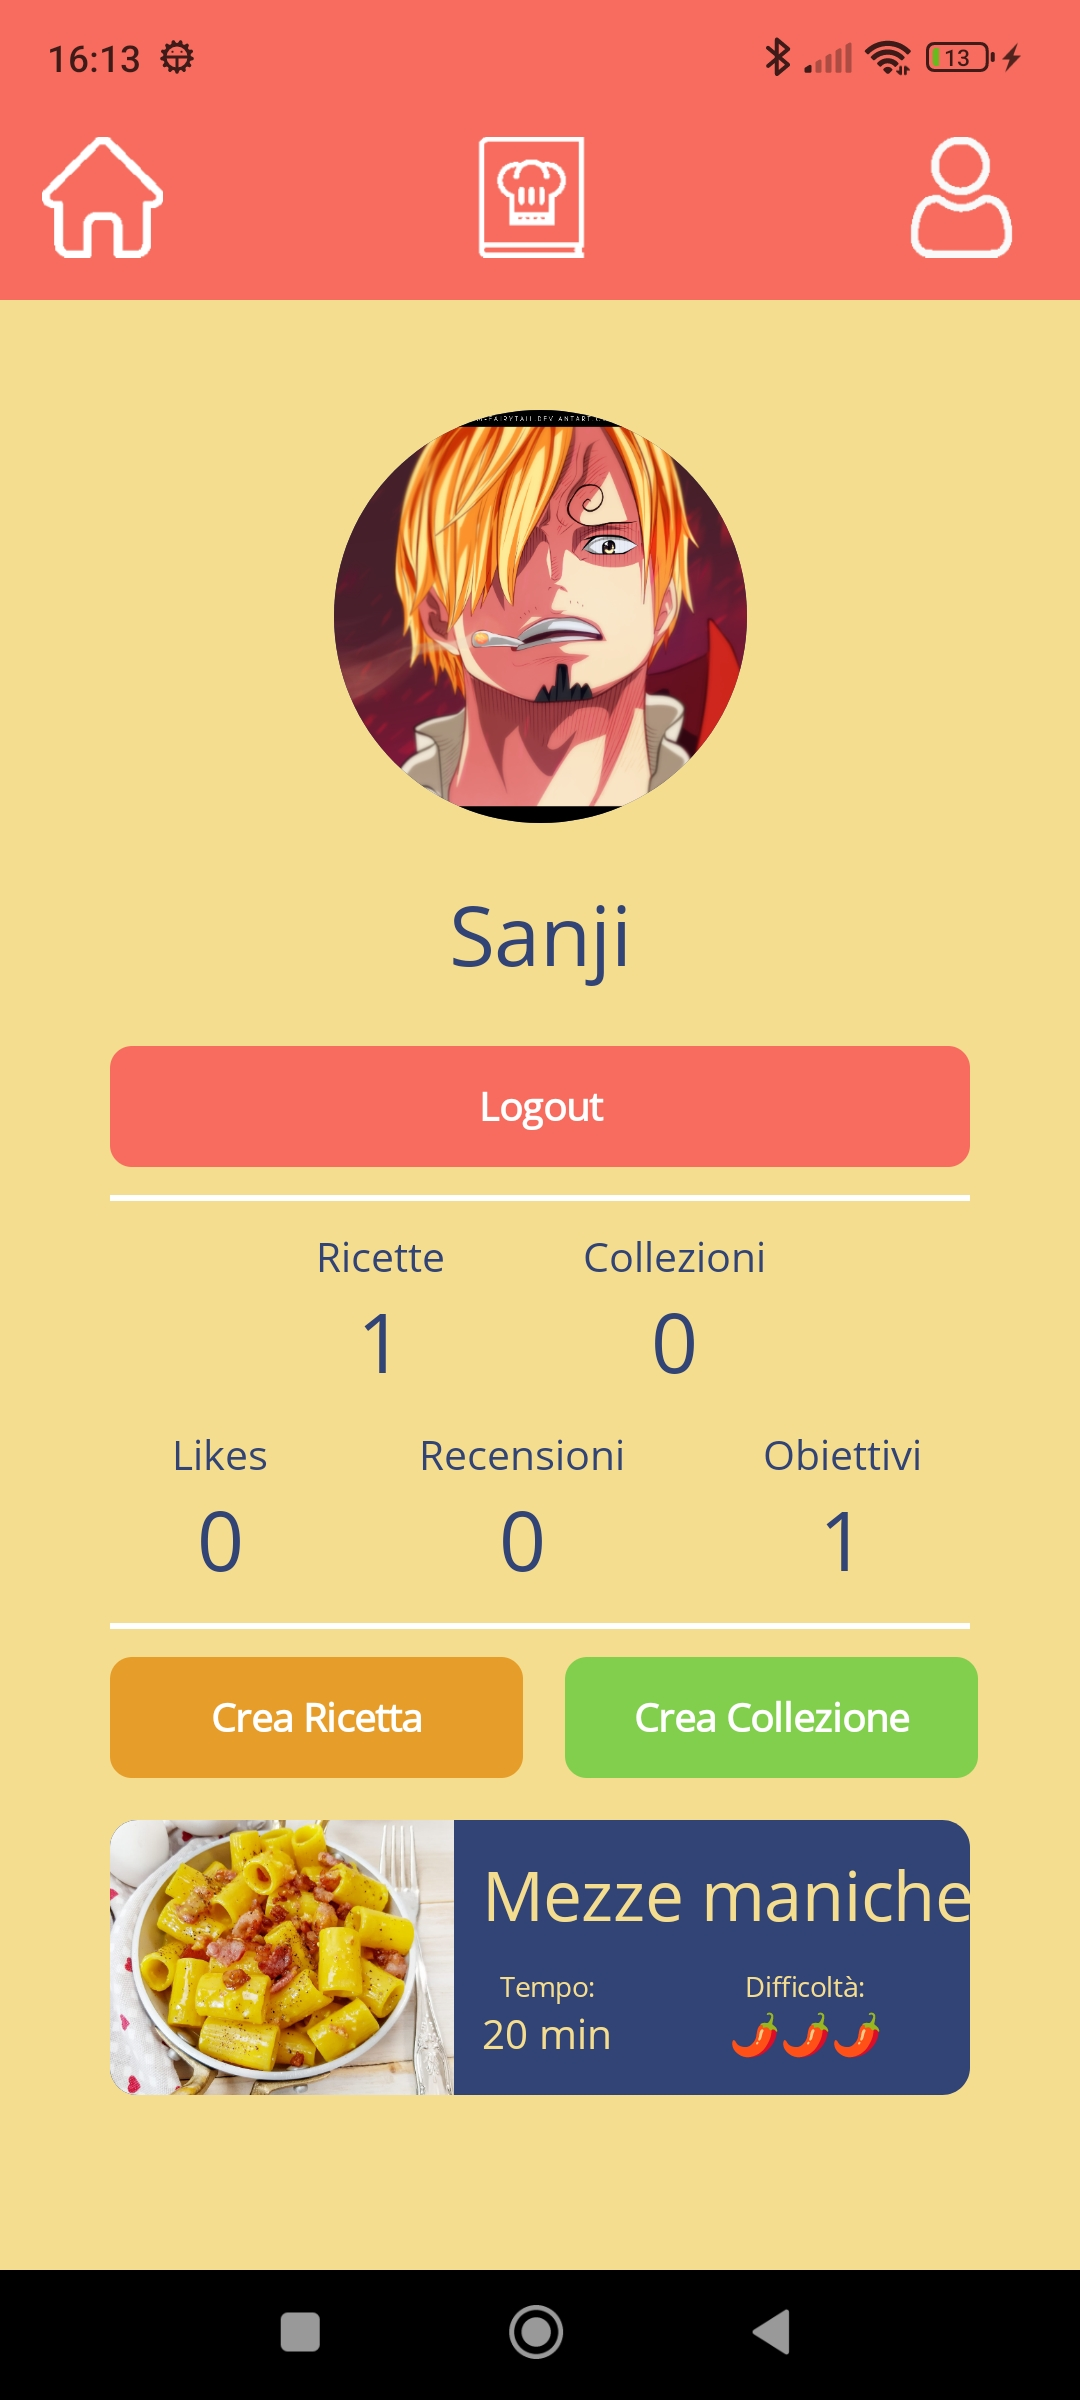
\includegraphics[width=0.4\linewidth]{app_images/UserPage.jpg}
\end{figure}
\\Clickando sul pulsante per la creazione di una ricetta comparirà la suddetta pagina con i vari campi da completare: 
\textbf{nome}, \textbf{descrizione}, \textbf{foto} (selezionandola dal proprio dispositivo), \textbf{lista dei passaggi} (scrivendo un passaggio alla volta e aggiungendolo alla lista), \textbf{difficoltà}, \textbf{tempo} e la \textbf{lista degli ingredienti} con la relativa quantità in grammi.\\
\begin{figure}[h!]
    \begin{minipage}{.5\textwidth}
        \centering
        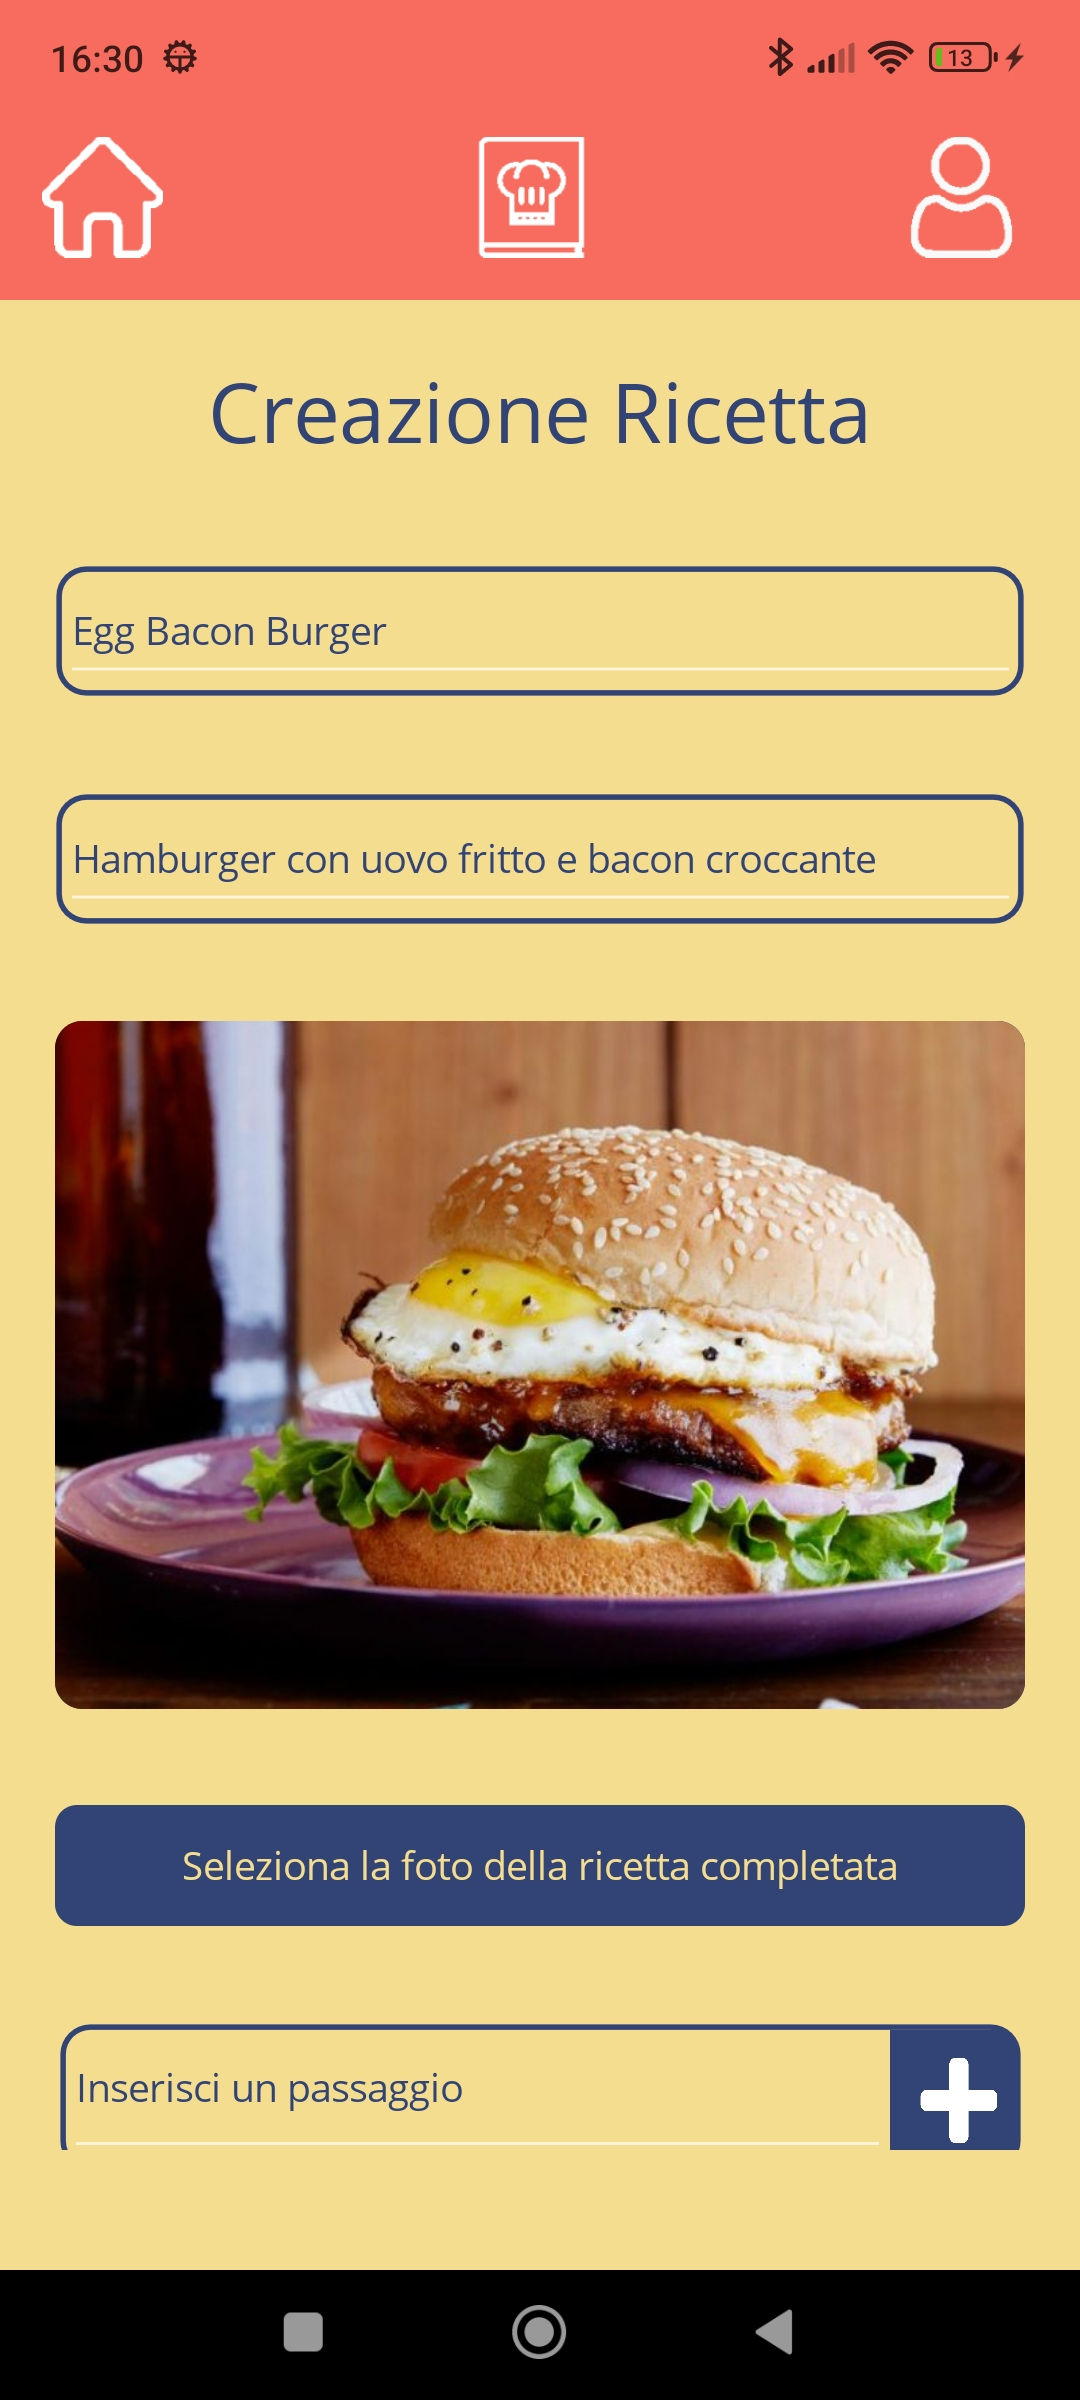
\includegraphics[width=0.9\linewidth]{app_images/RecipeCreation.jpg}
    \end{minipage}
    \begin{minipage}{.5\textwidth}
        \centering
        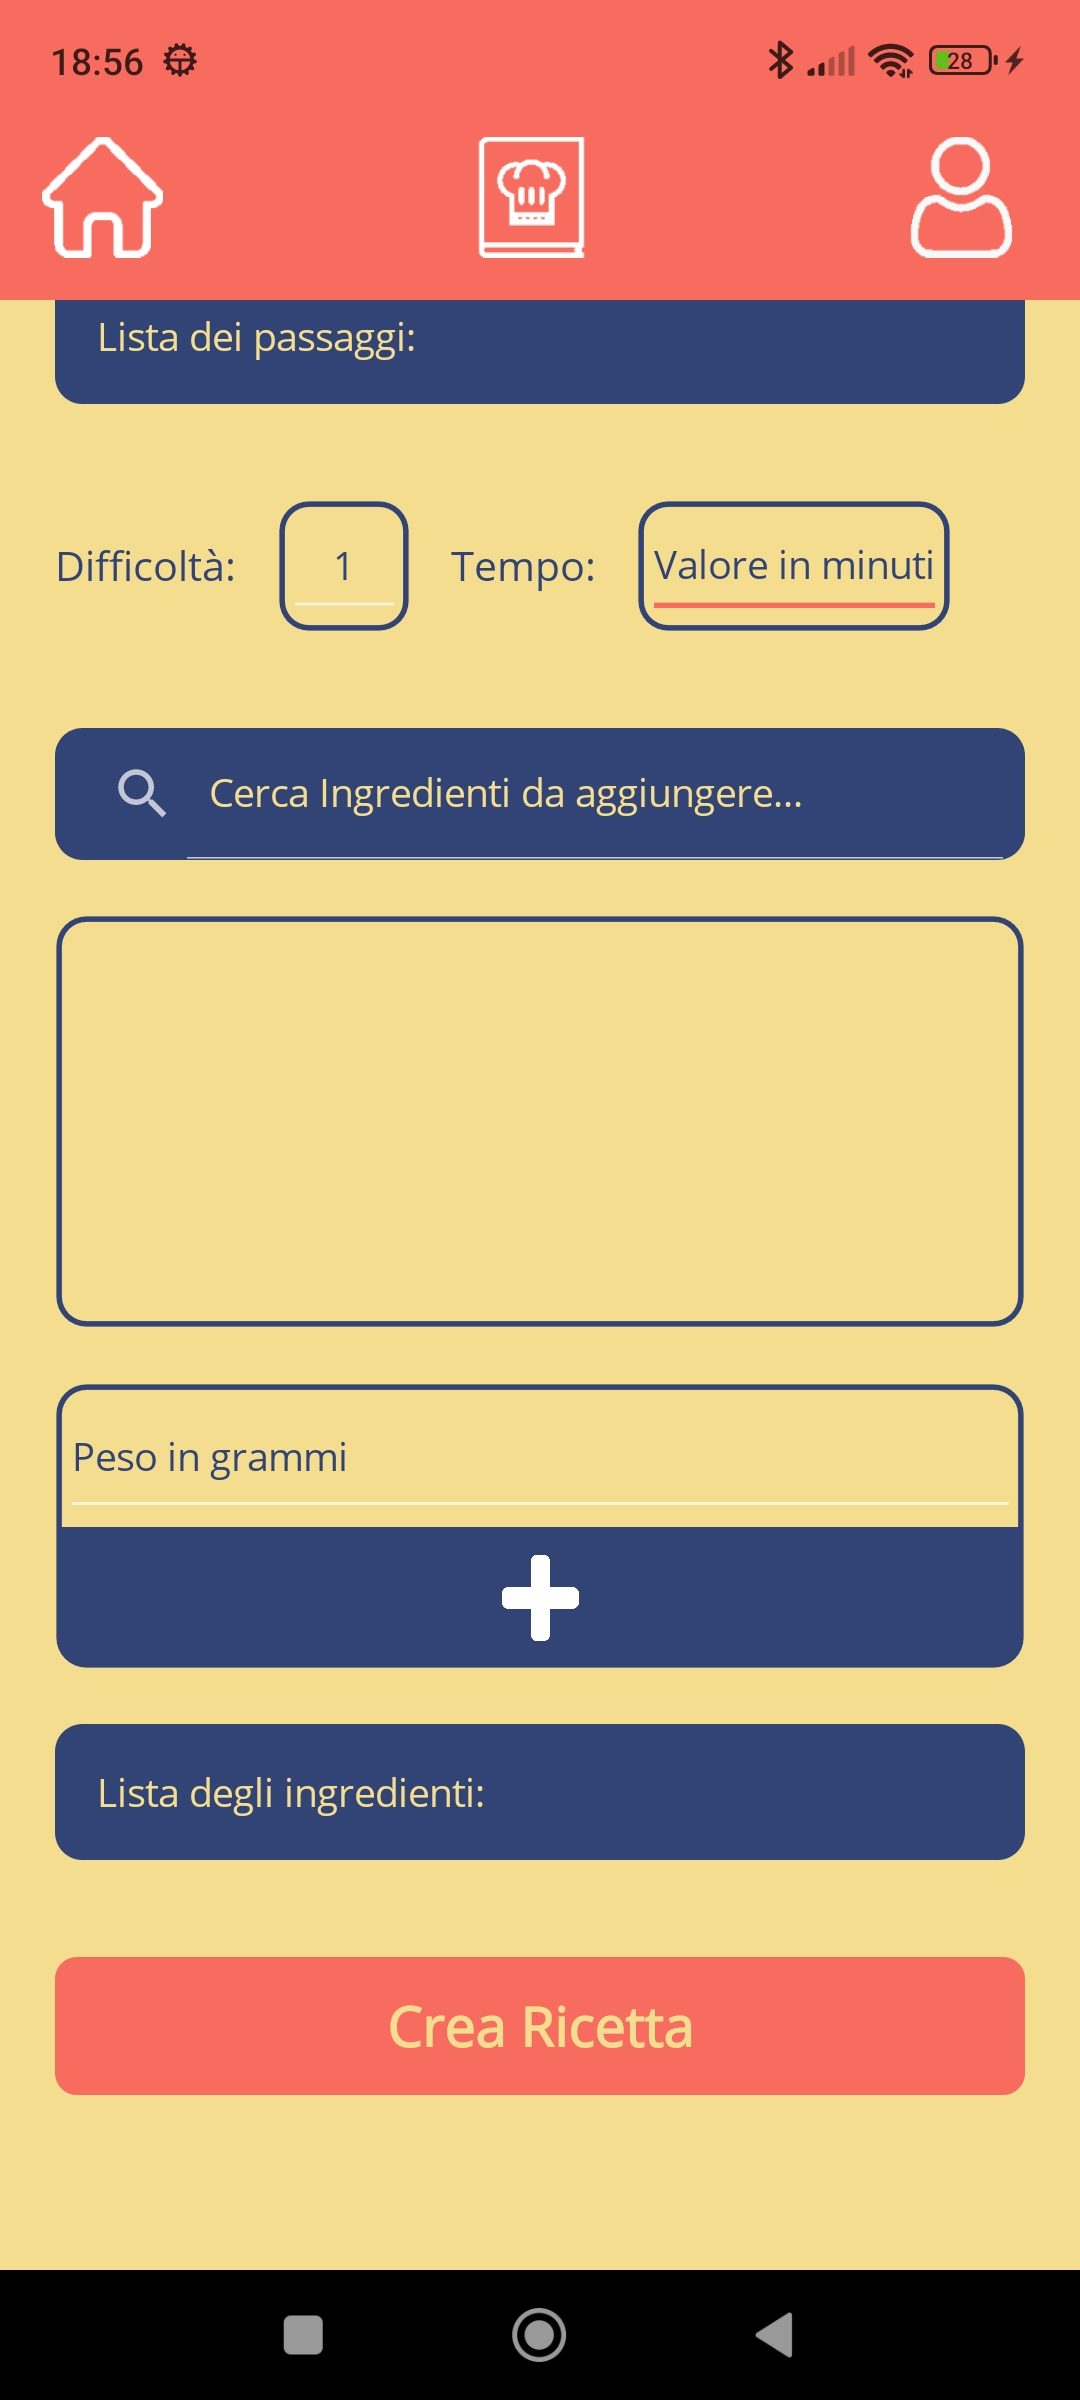
\includegraphics[width=0.9\linewidth]{app_images/RecipeCreation2.jpg}
    \end{minipage}
\end{figure}
\\\\\\\\\\\\\\Mentre clickando su quello per la creazione di collezioni/diete comparirà la pagina con i seguenti campi da completare:
\textbf{nome}, \textbf{descrizione}, checkbox per segnalare se si sta creando una \textbf{dieta} e scegliere la categoria nutrizionale e la \textbf{lista delle ricette} da aggiungere.
\begin{figure}[h!]
    \centering
    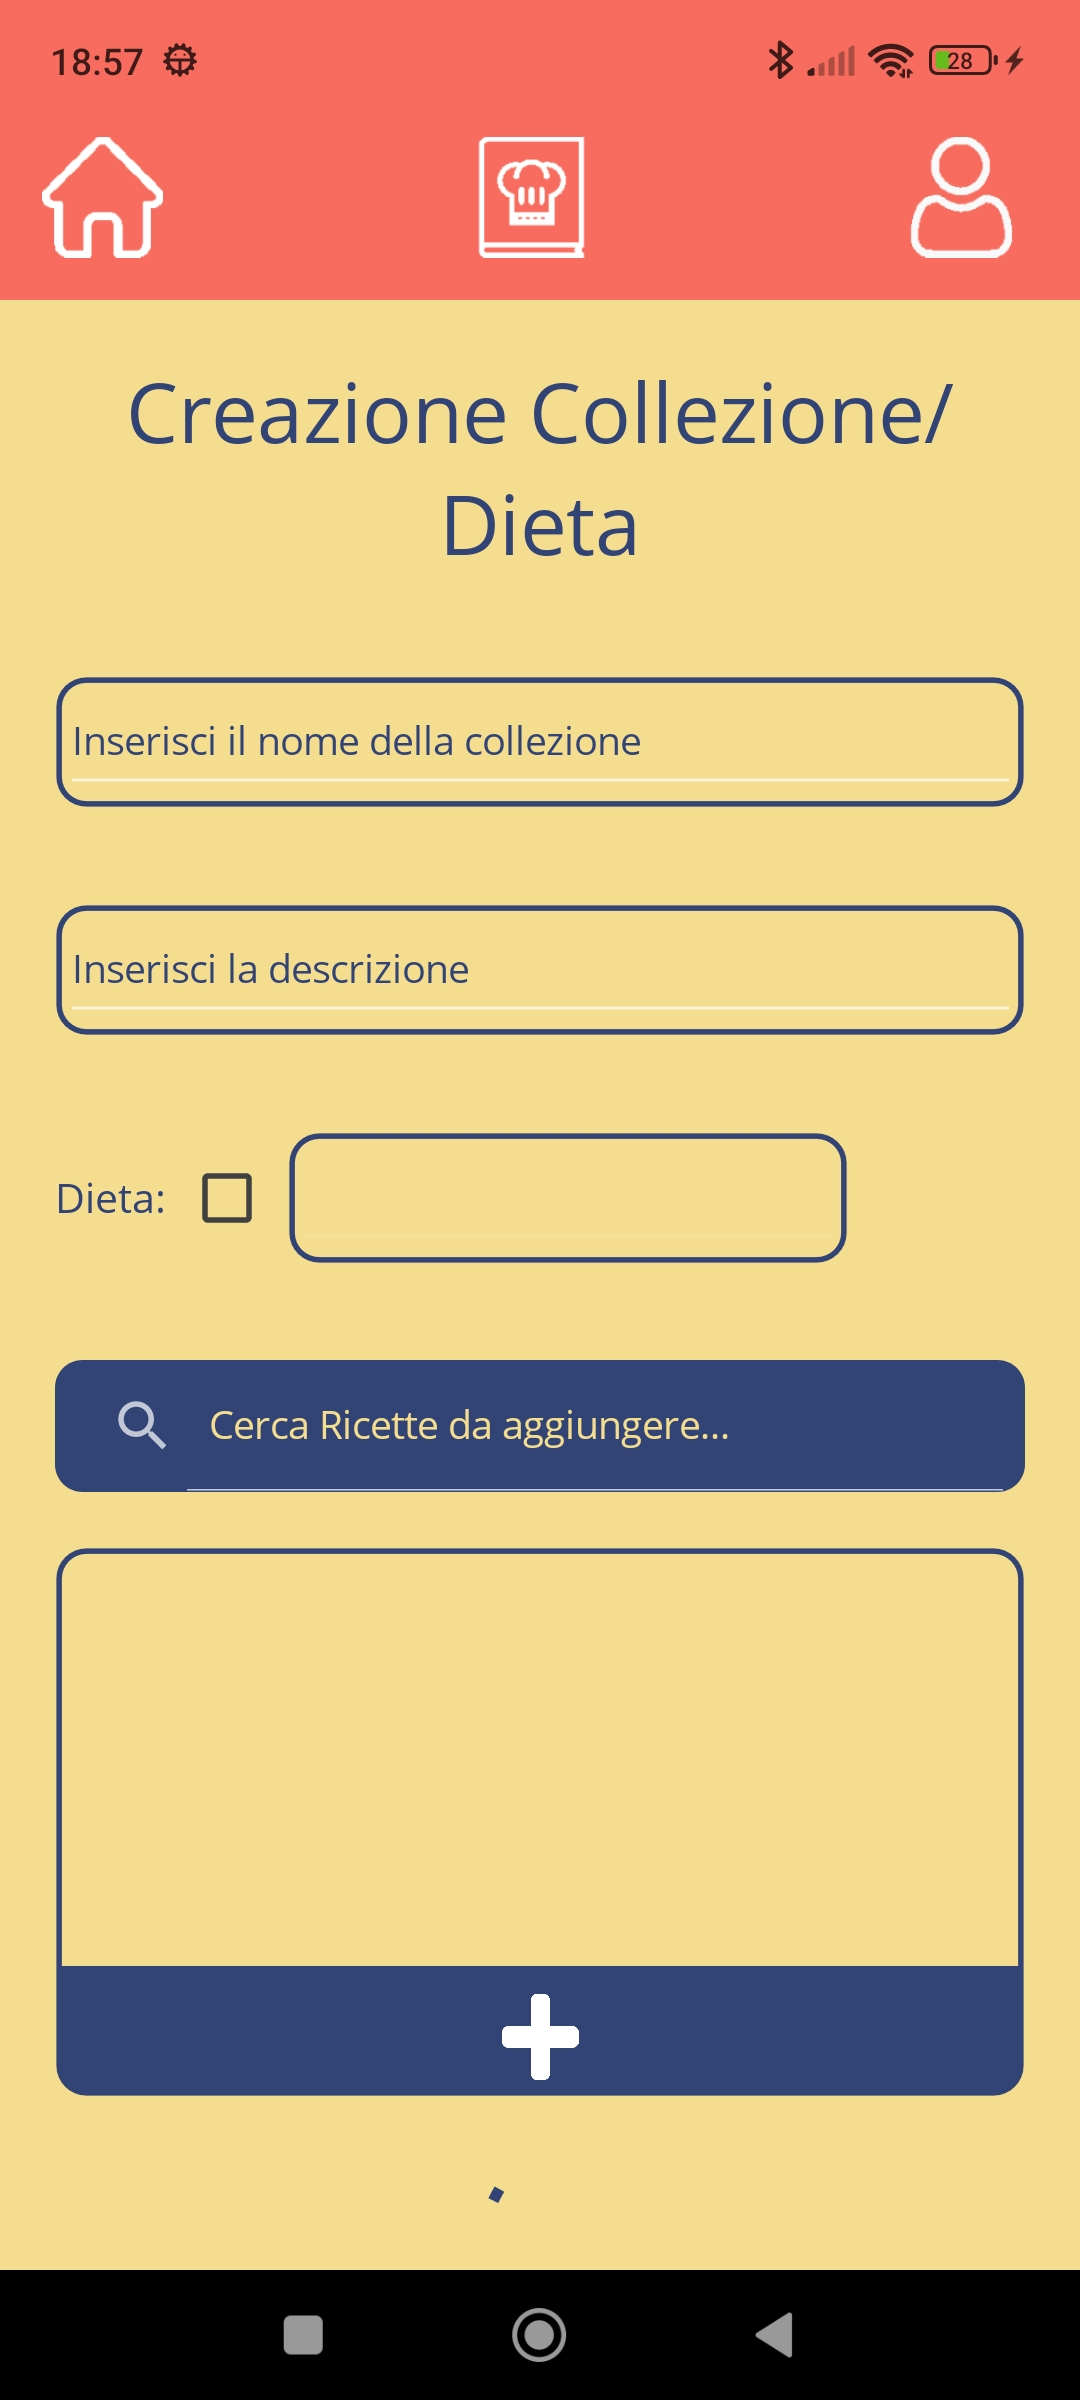
\includegraphics[width=0.5\linewidth]{app_images/CollectionCreation.jpg}
\end{figure}
\end{document}
